\documentclass[11pt,a4paper,oneside]{report}

% ==============================================================================
% PACCHETTI FONDAMENTALI
% ==============================================================================
\usepackage[utf8]{inputenc}
\usepackage[T1]{fontenc}
\usepackage[italian]{babel}
\usepackage{lmodern}
\usepackage{microtype}
\usepackage{graphicx}
\usepackage{caption}
\captionsetup{font={small,sf}, labelfont=bf}
\usepackage[top=2.5cm, bottom=2.5cm, left=2.5cm, right=2.5cm]{geometry}

% Matematica avanzata
\usepackage{amsmath,amssymb,amsthm,mathtools,bm}
\usepackage{mathrsfs}

% Tabelle e impaginazione
\usepackage{booktabs}
\usepackage{tabularx}
\usepackage{array}
\usepackage{multirow}
\usepackage{enumitem}
\usepackage{fancyhdr}
\usepackage{titlesec}

% Colori e Box grafici
\usepackage{xcolor}
\usepackage[most]{tcolorbox}

% Grafici TikZ e PGFPlots
\usepackage{tikz}
\usepackage{pgfplots}
\pgfplotsset{compat=1.18}
\usetikzlibrary{arrows.meta,calc,patterns,babel,decorations.pathreplacing}

% Configurazione per sistemi di equazioni con parentesi graffe ampie e proporzionate
\renewcommand{\arraystretch}{1.4}
\newenvironment{sistema}[1][1.5]{%
    \renewcommand{\arraystretch}{#1}%
    \left\{%
    \begin{array}{@{}l@{}}%
}{%
    \end{array}%
    \right.%
}

% Collegamenti ipertestuali
\usepackage[colorlinks=true,
            linkcolor=blue!80!black,
            citecolor=teal!80!black,
            urlcolor=cyan!80!black,
            bookmarksdepth=3]{hyperref}

% ==============================================================================
% DEFINIZIONE DELLA PALETTE COLORI ISTITUZIONALE
% ==============================================================================
\definecolor{primaryBlue}{RGB}{24, 76, 120}
\definecolor{accentTeal}{RGB}{18, 120, 115}
\definecolor{lightGray}{RGB}{245, 247, 250}
\definecolor{borderGray}{RGB}{209, 213, 219}
\definecolor{slateBorder}{RGB}{203, 213, 225}
\definecolor{alertRed}{RGB}{185, 28, 28}
\definecolor{accentRed}{RGB}{220, 38, 38}
\definecolor{warningAmber}{RGB}{217, 119, 6}
\definecolor{accentAmber}{RGB}{217, 119, 6}
\definecolor{examplePurple}{RGB}{109, 40, 217}
\definecolor{methodSlate}{RGB}{51, 65, 85}
\definecolor{rubricGreen}{RGB}{16, 122, 80}
\definecolor{accentGreen}{RGB}{22, 163, 74}

% ==============================================================================
% CONFIGURAZIONE AMBIENTI GRAFICI TCOLORBOX
% ==============================================================================

% 1. Definizione
\newtcolorbox[auto counter, number within=chapter]{definizione}[1][]{
    enhanced,
    colback=primaryBlue!5!white,
    colframe=primaryBlue,
    coltitle=white,
    fonttitle=\bfseries\sffamily,
    title=Definizione~\thetcbcounter\ifstrempty{#1}{}{: #1},
    sharp corners=northwest,
    arc=3mm,
    boxrule=1.2pt,
    top=3mm, bottom=3mm, left=4mm, right=4mm,
    before skip=4mm, after skip=4mm
}

% 2. Teorema
\newtcolorbox[auto counter, number within=chapter]{teorema}[1][]{
    enhanced,
    colback=accentTeal!6!white,
    colframe=accentTeal,
    coltitle=white,
    fonttitle=\bfseries\sffamily,
    title=Teorema~\thetcbcounter\ifstrempty{#1}{}{: #1},
    sharp corners=northwest,
    arc=3mm,
    boxrule=1.2pt,
    top=3mm, bottom=3mm, left=4mm, right=4mm,
    before skip=4mm, after skip=4mm
}

% 2b. Corollario
\newtcolorbox[auto counter, number within=chapter]{corollario}[1][]{
    enhanced,
    colback=accentTeal!4!white,
    colframe=accentTeal!80!black,
    coltitle=white,
    fonttitle=\bfseries\sffamily,
    title=Corollario~\thetcbcounter\ifstrempty{#1}{}{: #1},
    sharp corners=northwest,
    arc=3mm,
    boxrule=1pt,
    top=3mm, bottom=3mm, left=4mm, right=4mm,
    before skip=4mm, after skip=4mm
}

% 3. Dimostrazione
\newtcolorbox{dimostrazione}[1][Dimostrazione]{
    enhanced,
    blanker,
    breakable,
    left=4mm,
    before skip=3mm, after skip=4mm,
    borderline west={2.5pt}{0pt}{accentTeal!70!black},
    fontupper=\small,
    title={\bfseries\sffamily\color{accentTeal!80!black} #1.},
    attach title to upper={\par\vspace{1.5mm}}
}

% 4. Esercizio Svolto
\newtcolorbox[auto counter, number within=chapter]{esercizio}[1][]{
    enhanced,
    colback=examplePurple!5!white,
    colframe=examplePurple!90!black,
    coltitle=white,
    fonttitle=\bfseries\sffamily,
    title=Esercizio Svolto~\thetcbcounter\ifstrempty{#1}{}{: #1},
    arc=2mm,
    boxrule=1pt,
    top=3mm, bottom=3mm, left=4mm, right=4mm,
    before skip=4mm, after skip=4mm
}

% 5. Esempio
\newtcolorbox[auto counter, number within=chapter]{esempio}[1][]{
    enhanced,
    colback=warningAmber!6!white,
    colframe=warningAmber!90!black,
    coltitle=white,
    fonttitle=\bfseries\sffamily,
    title=Esempio Guida~\thetcbcounter\ifstrempty{#1}{}{: #1},
    arc=2mm,
    boxrule=1pt,
    top=3mm, bottom=3mm, left=4mm, right=4mm,
    before skip=4mm, after skip=4mm
}

% 6. Attenzione / Errore Didattico Frequente
\newtcolorbox{attenzione}[1][Attenzione: Errore Ricorrente]{
    enhanced,
    colback=alertRed!6!white,
    colframe=alertRed,
    coltitle=white,
    fonttitle=\bfseries\sffamily,
    title=\textbf{#1},
    arc=2mm,
    boxrule=1.2pt,
    top=3mm, bottom=3mm, left=4mm, right=4mm,
    before skip=4mm, after skip=4mm
}

% 7. Metodo Operativo / Schema di Calcolo
\newtcolorbox{metodo}[1][Schema Metodologico]{
    enhanced,
    colback=methodSlate!5!white,
    colframe=methodSlate,
    coltitle=white,
    fonttitle=\bfseries\sffamily,
    title=#1,
    arc=2mm,
    boxrule=1.2pt,
    top=3mm, bottom=3mm, left=4mm, right=4mm,
    before skip=4mm, after skip=4mm
}


% ==============================================================================
% CONFIGURAZIONE HEADER E FOOTER
% ==============================================================================
\pagestyle{fancy}
\fancyhf{}
\fancyhead[L]{\small\sffamily\color{gray}Quaderno del Prof -- Classe 4B}
\fancyhead[R]{\small\sffamily\color{gray}Esponenziali, Logaritmi e Goniometria}
\fancyfoot[C]{\small\sffamily\thepage}
\renewcommand{\headrulewidth}{0.4pt}
\renewcommand{\footrulewidth}{0pt}

% Titoli delle sezioni con font sans-serif elegante
\titleformat{\chapter}[display]
  {\normalfont\sffamily\huge\bfseries\color{primaryBlue}}
  {\chaptertitlename\ \thechapter}{15pt}{\Huge}
\titleformat{\section}
  {\normalfont\sffamily\Large\bfseries\color{primaryBlue}}
  {\thesection}{1em}{}
\titleformat{\subsection}
  {\normalfont\sffamily\large\bfseries\color{accentTeal}}
  {\thesubsection}{1em}{}

% ==============================================================================
% INIZIO DOCUMENTO
% ==============================================================================
\begin{document}

% ------------------------------------------------------------------------------
% FRONTESPIZIO
% ------------------------------------------------------------------------------
\begin{titlepage}
    \centering
    \vspace*{2.0cm}
    
    {\fontsize{34}{42}\selectfont\sffamily\bfseries\color{primaryBlue} Quaderno del Prof}\\[0.6cm]
    {\Large\sffamily\bfseries\color{accentTeal} Matematica}\\[0.3cm]
    {\large\sffamily\color{methodSlate} Teoria Completa, Dimostrazioni Passo-Passo ed Esercizi Risolti}\\[1.5cm]
    
    \rule{0.85\linewidth}{1.5pt}\\[1.5cm]
    
    {\huge\sffamily\bfseries ESPONENZIALI, LOGARITMI\\ E INTRODUZIONE ALLA GONIOMETRIA}\\[1.5cm]
    
    \rule{0.85\linewidth}{1.5pt}\\[2.0cm]
    
    {\Large\sffamily
    \textbf{Liceo Scientifico Statale «Leonardo da Vinci» -- Maglie}\\[0.3cm]
    Classe: \textbf{4ª Sezione B}\\[0.2cm]
    Materia: \textbf{Matematica}
    }
    
    \vfill
\end{titlepage}

% ------------------------------------------------------------------------------
% INDICE GENERALE
% ------------------------------------------------------------------------------
\tableofcontents
\newpage

% ==============================================================================
% CAPITOLO 1: FUNZIONE ESPONENZIALE E COSTANTE DI NEPERO
% ==============================================================================
\chapter{La Funzione Esponenziale e la Costante di Nepero}

\section{La Genesi del Numero \texorpdfstring{$e$}{e}: Il Problema di Jacob Bernoulli}
Il numero trascendente $e \approx 2{,}718281828459\dots$, noto storicamente come \emph{costante di Eulero} o \emph{numero di Nepero}, trae la propria origine formale dall'analisi finanziaria della capitalizzazione composta intrapresa dal matematico svizzero Jacob Bernoulli nel 1683.

Consideriamo un capitale iniziale $C$ investito a un tasso nominale di rendimento annuo pari al $100\%$ ($r = 1$). Se l'interesse viene riconosciuto e liquidato esclusivamente alla fine dell'anno (capitalizzazione semplice annuale), il montante finale $M$ generato è:
\begin{equation}
    M = C + C \cdot 1 = C(1 + 1) = 2C
\end{equation}
Qualora il medesimo rendimento annuale venga frazionato in due semestri, a ciascuna scadenza semestrale corrisponderà un tasso parziale pari a $\frac{r}{2} = 50\% = 0{,}5$. Al termine del primo semestre il capitale accumulato diventa:
\begin{equation}
    M_{1/2} = C + C \cdot 0{,}5 = C(1 + 0{,}5) = 1{,}5 \, C
\end{equation}
Nel secondo semestre, l'interesse non matura solo sul capitale primitivo $C$, bensì sull'intero montante $M_{1/2}$ maturato (regime di interesse composto):
\begin{equation}
    M_1 = M_{1/2} + M_{1/2} \cdot 0{,}5 = M_{1/2}(1 + 0{,}5) = C(1 + 0{,}5)(1 + 0{,}5) = C\left(1 + \frac{1}{2}\right)^2 = 2{,}25 \, C
\end{equation}
Generalizzando il procedimento a una suddivisione dell'anno in $n$ sotto-periodi omogenei (quadrimestri con $n=3$, trimestri con $n=4$, mesi con $n=12$, giorni con $n=365$), il tasso per ciascun periodo è $\frac{1}{n}$ e il montante finale dopo un anno è governato dalla legge:
\begin{equation}
    M_n = C\left(1 + \frac{1}{n}\right)^n
\end{equation}

\begin{table}[htbp]
\centering
\small
\caption{Convergenza del montante $M_n$ per $C = 1000\text{ euro}$ al crescere delle frazioni temporali $n$.}
\label{tab:bernoulli}
\begin{tabularx}{\textwidth}{l c >{\centering\arraybackslash}X r}
\toprule
\textbf{Frequenza} & \textbf{Periodi ($n$)} & \textbf{Formula analitica} & \textbf{Montante finale (EUR)} \\
\midrule
Annuale & $n = 1$ & $1000 \cdot (1 + 1)^1$ & $2000{,}00$ \\
Semestrale & $n = 2$ & $1000 \cdot (1 + 0{,}5)^2$ & $2250{,}00$ \\
Quadrimestrale & $n = 3$ & $1000 \cdot (1 + 1/3)^3$ & $2370{,}37$ \\
Trimestrale & $n = 4$ & $1000 \cdot (1 + 0{,}25)^4$ & $2441{,}41$ \\
Mensile & $n = 12$ & $1000 \cdot (1 + 1/12)^{12}$ & $2613{,}04$ \\
Giornaliero & $n = 365$ & $1000 \cdot (1 + 1/365)^{365}$ & $2714{,}57$ \\
Orario & $n = 8760$ & $1000 \cdot (1 + 1/8760)^{8760}$ & $2718{,}13$ \\
Al secondo & $n = 31\,536\,000$ & $1000 \cdot (1 + 1/n)^n$ & $2718{,}28$ \\
\textbf{Continua (istante per istante)} & \textbf{Stabilizzazione} & $\mathbf{1000 \cdot e}$ & $\mathbf{2718{,}2818\dots}$ \\
\bottomrule
\end{tabularx}
\end{table}

\begin{figure}[htbp]
\centering
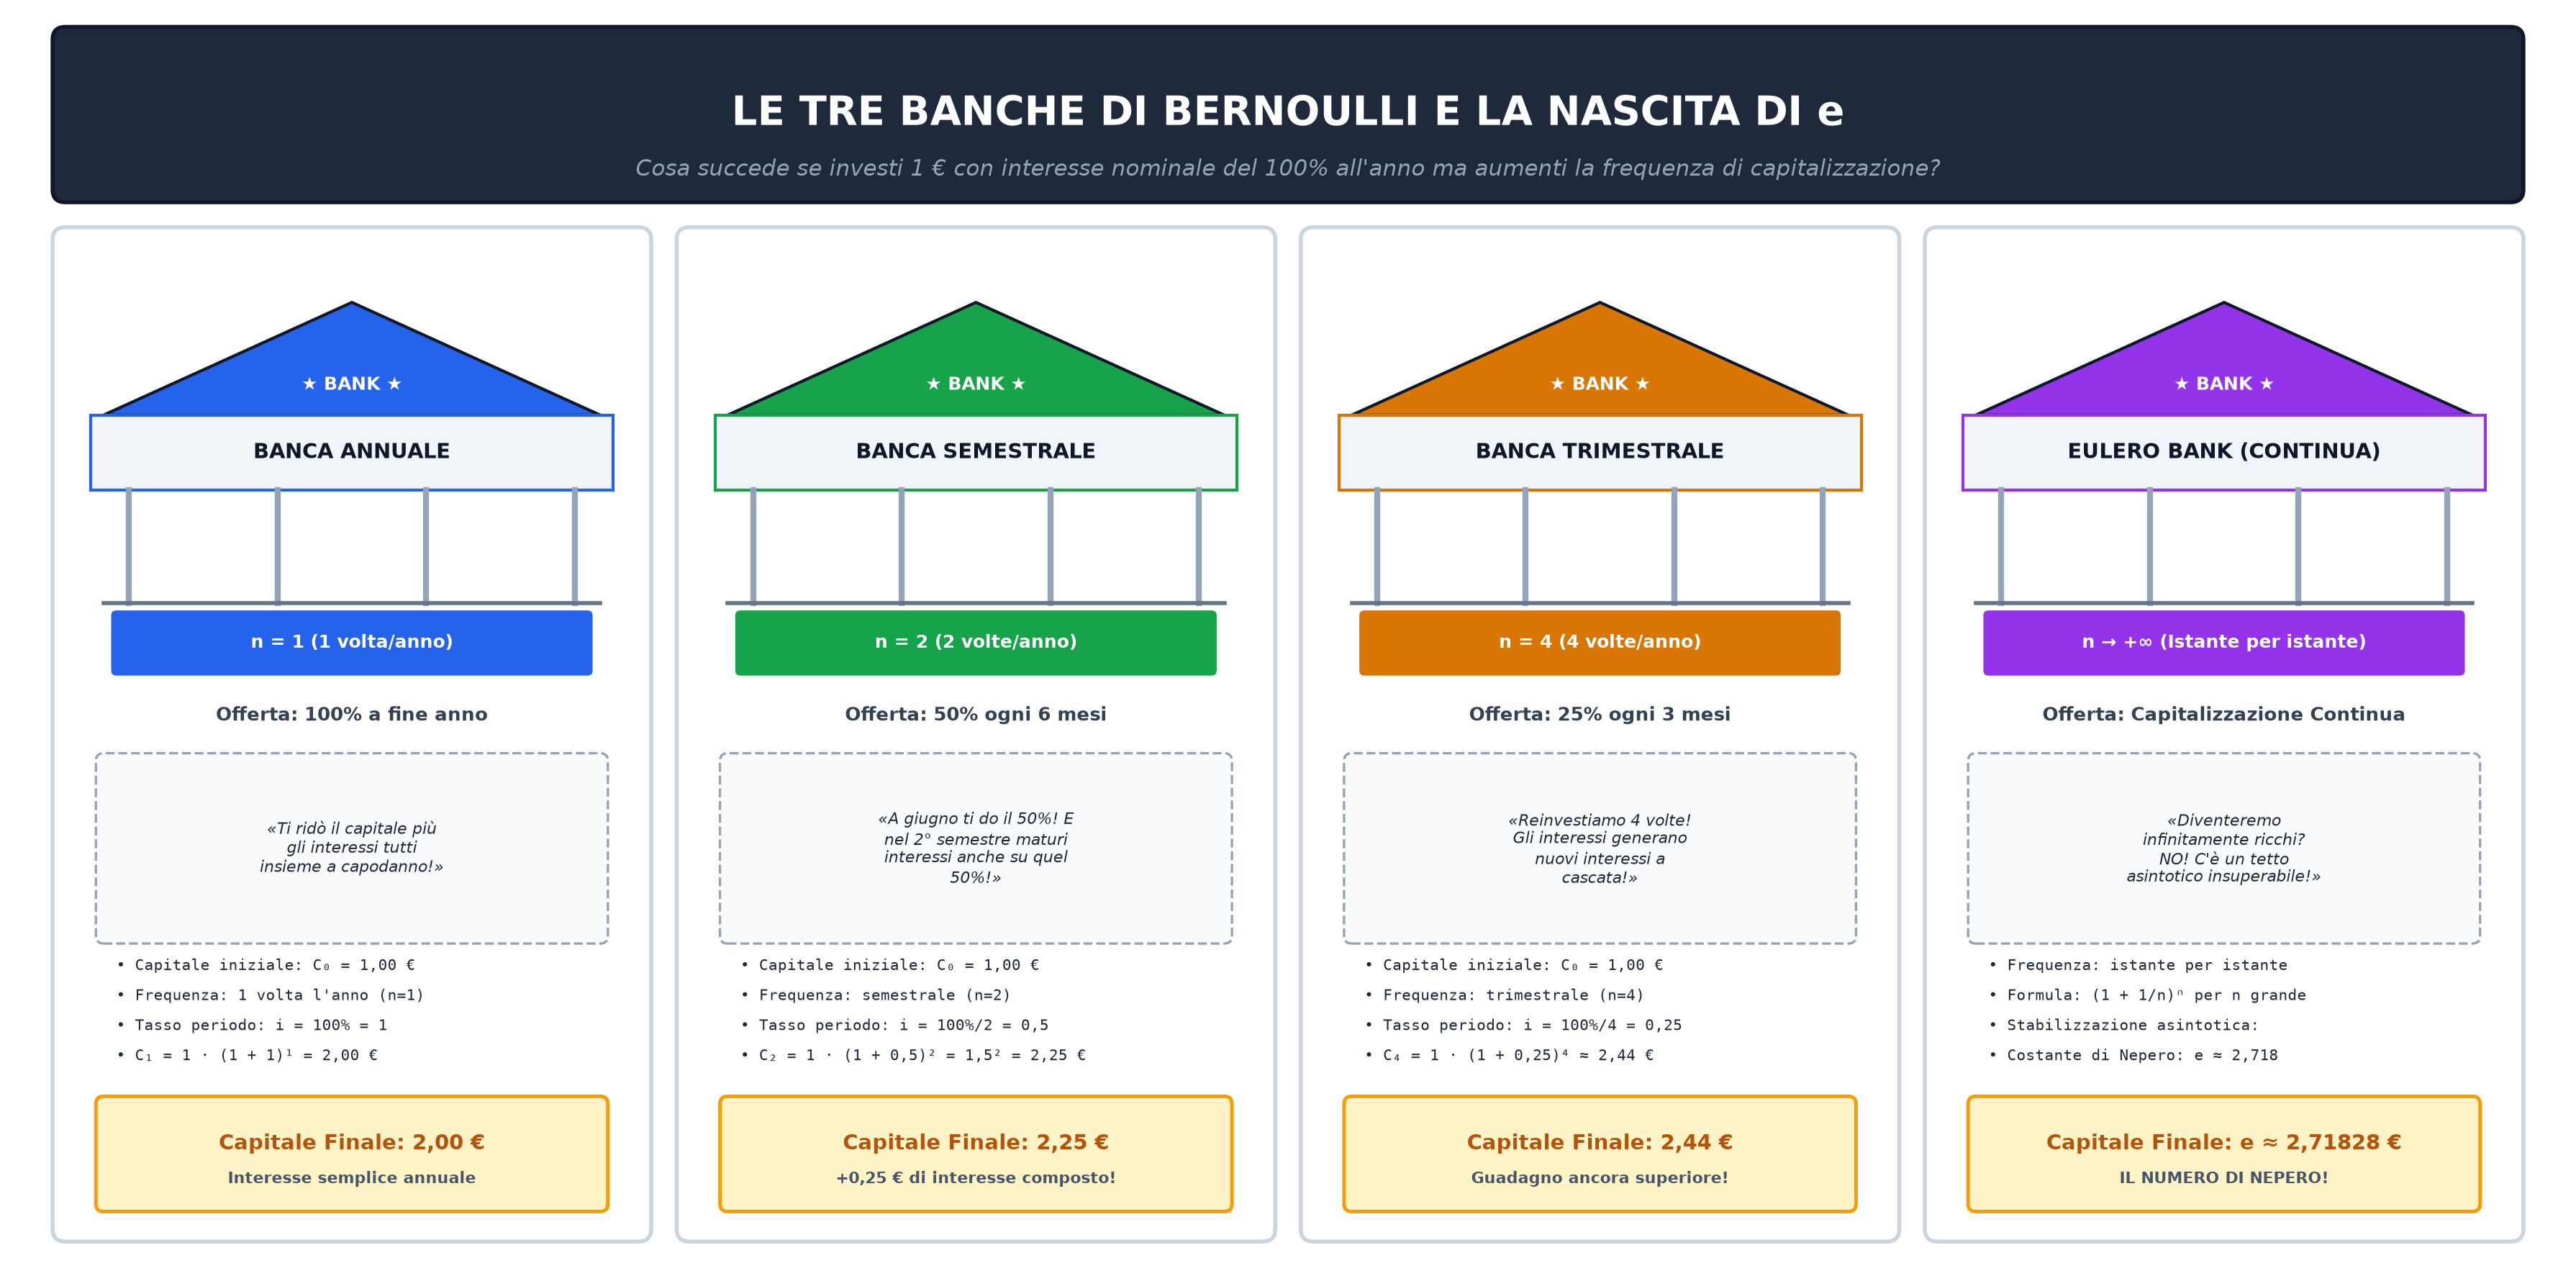
\includegraphics[width=0.96\textwidth]{immagini/bernoulli_banche_fumetto.png}
\caption{Striscia e infografica didattica: Il paradosso economico di Jacob Bernoulli e il confronto tra le banche (annuale 100\%, semestrale 50\%, trimestrale 25\%) fino alla soglia asintotica insuperabile del numero di Nepero $e \approx 2{,}71828\dots\text{ EUR}$.}
\label{fig:banche_bernoulli}
\end{figure}

\begin{teorema}[La Costante di Nepero $e$]
All'aumentare indefinito del numero $n$ di suddivisioni temporali nella capitalizzazione composta, i valori della successione:
\begin{equation}
    a_n = \left(1 + \frac{1}{n}\right)^n, \quad n \in \mathbb{N}^+
\end{equation}
crescono progressivamente mantenendosi sempre inferiori a $3$. La successione si stabilizza così verso un valore numerico costante e insuperabile, indicato universalmente con la lettera $e$:
\begin{equation}
    e \approx 2{,}718281828459\dots
\end{equation}
\end{teorema}

\begin{dimostrazione}[\bfseries Dimostrazione Analitica: Monotonia e Limitatezza $a_n < 3$ con il Binomio di Newton]
Utilizzando lo sviluppo del binomio di Newton:
\begin{align*}
    a_n &= \left(1 + \frac{1}{n}\right)^n = \sum_{k=0}^n \binom{n}{k} \frac{1}{n^k} \\
    &= 1 + n \cdot \frac{1}{n} + \frac{n(n-1)}{2!} \frac{1}{n^2} + \frac{n(n-1)(n-2)}{3!} \frac{1}{n^3} + \dots + \frac{n(n-1)\dots 1}{n!} \frac{1}{n^n} \\
    &= 1 + 1 + \frac{1}{2!}\left(1 - \frac{1}{n}\right) + \frac{1}{3!}\left(1 - \frac{1}{n}\right)\left(1 - \frac{2}{n}\right) + \dots + \frac{1}{n!}\left(1 - \frac{1}{n}\right)\dots\left(1 - \frac{n-1}{n}\right)
\end{align*}
Ciascun addendo è positivo. All'aumentare di $n$ a $n+1$, compaiono sia un termine aggiuntivo positivo, sia fattori moltiplicativi $\left(1 - \frac{k}{n}\right) < \left(1 - \frac{k}{n+1}\right)$ più grandi. Dunque $a_n < a_{n+1}$ (stretta crescenza).

Inoltre, poiché $\left(1 - \frac{k}{n}\right) < 1$ e per $k \ge 2$ si ha $k! \ge 2^{k-1}$:
\begin{equation}
    a_n < 1 + 1 + \frac{1}{2!} + \frac{1}{3!} + \dots + \frac{1}{n!} < 1 + 1 + \frac{1}{2} + \frac{1}{4} + \dots + \frac{1}{2^{n-1}} = 1 + \frac{1 - (1/2)^n}{1 - 1/2} < 1 + 2 = 3
\end{equation}
Essendo monotona crescente e limitata superiormente da 3, i valori della successione si stabilizzano e convergono a un valore finito compreso tra $2$ e $3$, identificato con la costante $e$.
\end{dimostrazione}

\section{Algebra delle Potenze ad Esponente Reale}
Prima di analizzare la funzione esponenziale reale, richiamiamo le proprietà fondamentali delle potenze. Siano $a, b \in \mathbb{R}^+$ ed $x, y \in \mathbb{R}$:
\begin{enumerate}[label=\textbf{\arabic*.}]
    \item $a^x \cdot a^y = a^{x+y}$
    \item $\dfrac{a^x}{a^y} = a^{x-y}$
    \item $(a^x)^y = a^{x \cdot y}$
    \item $(a \cdot b)^x = a^x \cdot b^x$
    \item $\left(\dfrac{a}{b}\right)^x = \dfrac{a^x}{b^x}$
    \item $a^{-x} = \dfrac{1}{a^x}$
    \item $a^{m/n} = \sqrt[n]{a^m} \quad (m \in \mathbb{Z}, n \in \mathbb{N}^+)$
\end{enumerate}

\section{Definizione e Proprietà della Funzione Esponenziale}

\begin{definizione}[Funzione Esponenziale]
Si definisce \emph{funzione esponenziale elementare di base $a$} l'applicazione:
\begin{equation}
    f \colon \mathbb{R} \to \mathbb{R}^+, \quad f(x) = a^x
\end{equation}
con il vincolo fondamentale di ammissibilità della base:
\begin{equation}
    a > 0 \quad \text{e} \quad a \neq 1
\end{equation}
\end{definizione}

\begin{attenzione}[Perché la base $a$ deve soddisfare $a > 0$ ed $a \neq 1$?]
\begin{itemize}
    \item Se $a < 0$: l'espressione $a^x$ perde di significato reale per infiniti esponenti frazionari. Ad esempio, per $a = -4$ e $x = 1/2$, si avrebbe $(-4)^{1/2} = \sqrt{-4} \notin \mathbb{R}$. La funzione non sarebbe definibile in un intervallo continuo.
    \item Se $a = 0$: si avrebbe $0^x = 0$ per ogni $x > 0$, mentre per $x \le 0$ l'espressione risulterebbe indeterminata ($0^0$) o priva di significato ($0^{-1} = 1/0$).
    \item Se $a = 1$: l'espressione $1^x = 1$ degenera nella retta orizzontale costante $y = 1$, perdendo la caratteristica di biiettività essenziale per definire il logaritmo.
\end{itemize}
\end{attenzione}

\subsection{Caratteristiche Analitiche e Asintoti}
\begin{itemize}
    \item \textbf{Dominio:} $\mathcal{D} = \mathbb{R} = (-\infty, +\infty)$.
    \item \textbf{Codominio (Insieme Immagine):} $\mathrm{Im}(f) = \mathbb{R}^+ = (0, +\infty)$. L'esponenziale reale è sempre strettamente positiva:
    \begin{equation}
        a^x > 0 \quad \forall x \in \mathbb{R}
    \end{equation}
    \item \textbf{Punto fisso fondamentale:} Per ogni $a$, si ha $a^0 = 1$, dunque il grafico interseca l'asse delle ordinate nel punto $P(0, 1)$. Inoltre passa per $(1, a)$.
    \item \textbf{Biforcazione della monotonia:}
    \begin{itemize}
        \item Se $\mathbf{a > 1}$: la funzione è \textbf{strettamente crescente}:
        \begin{equation}
            x_1 < x_2 \iff a^{x_1} < a^{x_2}
        \end{equation}
        Comportamento asintotico e andamento globale:
        \begin{itemize}
            \item Per valori di $x$ negativi di modulo sempre più grande ($x \to -\infty$), i valori di $a^x$ si avvicinano sempre più alla retta $y = 0$ senza mai toccarla (\textbf{asintoto orizzontale sinistro}: $y = 0$).
            \item Per valori di $x$ positivi via via crescenti ($x \to +\infty$), i valori di $a^x$ crescono indefinitamente verso l'alto ($y \to +\infty$).
        \end{itemize}
        \item Se $\mathbf{0 < a < 1}$: la funzione è \textbf{strettamente decrescente}:
        \begin{equation}
            x_1 < x_2 \iff a^{x_1} > a^{x_2}
        \end{equation}
        Comportamento asintotico e andamento globale:
        \begin{itemize}
            \item Per valori di $x$ negativi di modulo sempre più grande ($x \to -\infty$), i valori della funzione crescono indefinitamente verso l'alto ($y \to +\infty$).
            \item All'aumentare indefinito di $x$ verso valori positivi ($x \to +\infty$), la curva si avvicina sempre più alla retta $y = 0$ senza mai toccarla (\textbf{asintoto orizzontale destro}: $y = 0$).
        \end{itemize}
    \end{itemize}
    \item \textbf{Simmetria speculare tra basi reciproche:} Poiché $\left(\frac{1}{a}\right)^x = a^{-x}$, la curva $y = \left(\frac{1}{a}\right)^x$ si ottiene da $y = a^x$ mediante una riflessione assiale rispetto all'asse delle ordinate $y$ ($x \mapsto -x$).
\end{itemize}

\section{Rappresentazione Grafica Comparativa}

\begin{figure}[htbp]
\centering
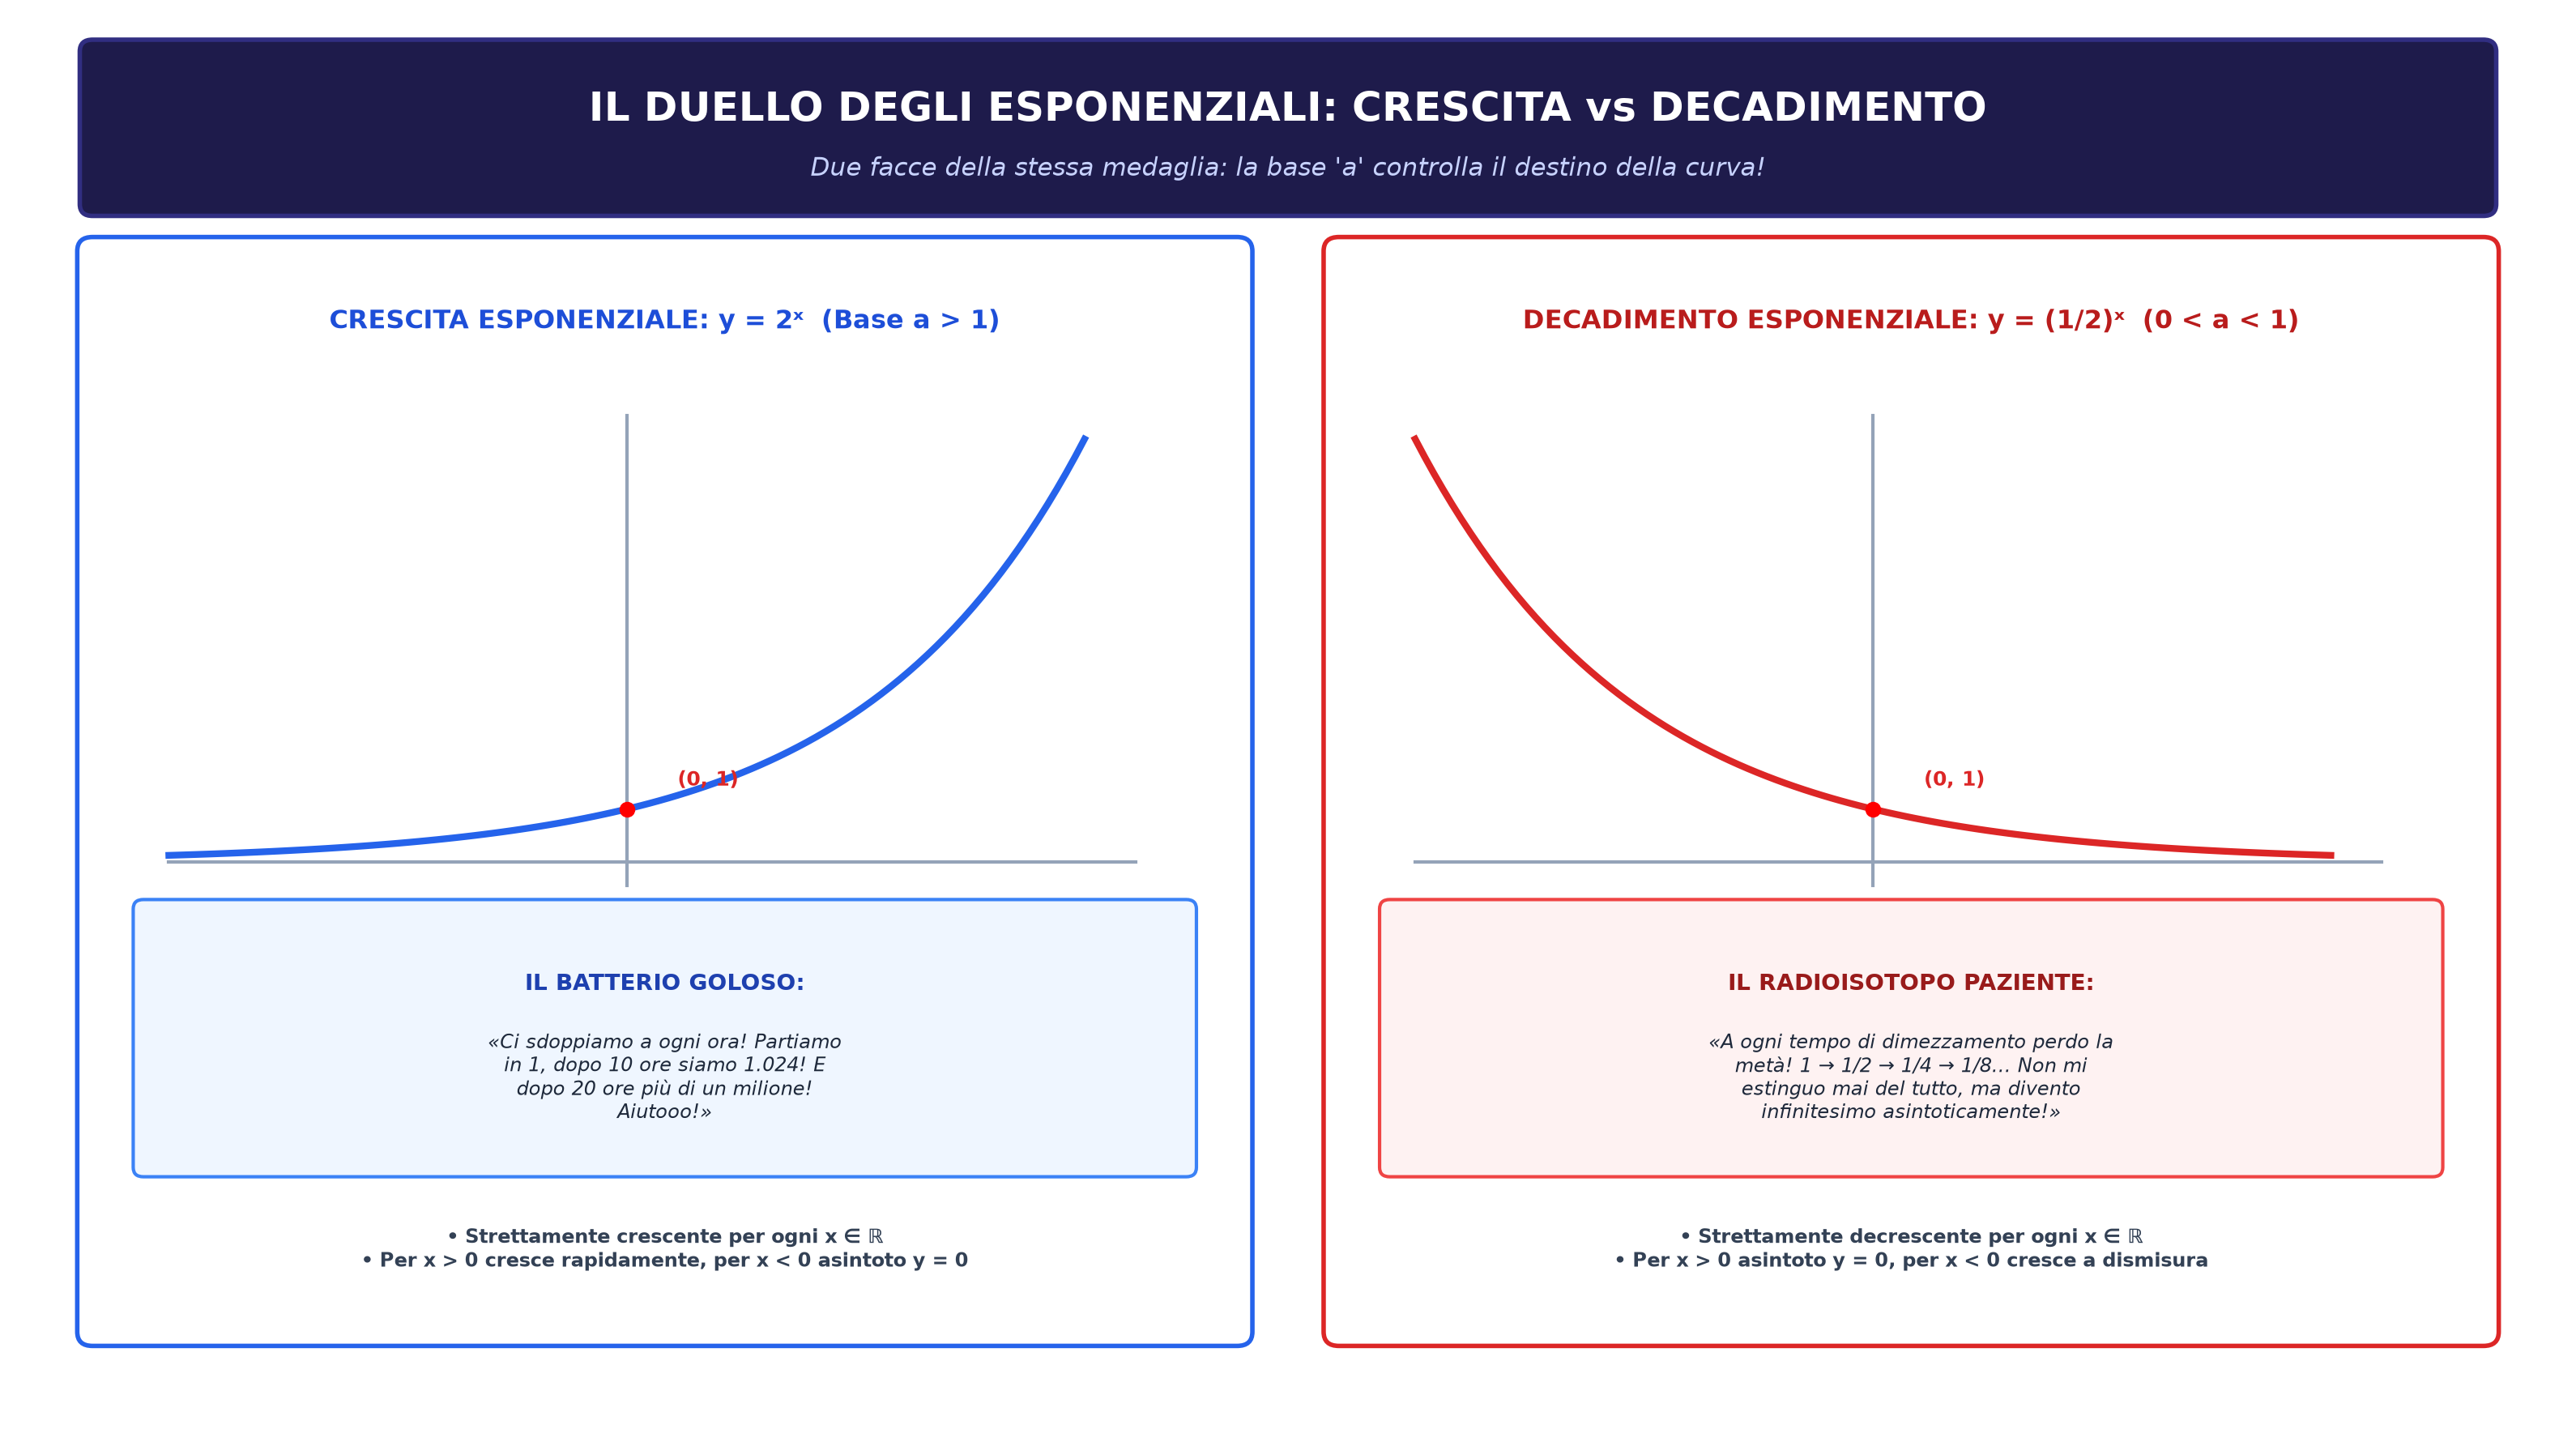
\includegraphics[width=0.92\textwidth]{immagini/duello_esponenziali.png}
\caption{Infografica comparativa: Il duello degli esponenziali. La base $a > 1$ governa la moltiplicazione esponenziale ($y = 2^x$), mentre $0 < a < 1$ governa il decadimento asintotico a tempo di dimezzamento ($y = (1/2)^x$).}
\label{fig:duello_esponenziali}
\end{figure}

\begin{figure}[htbp]
\centering
\begin{tikzpicture}
\begin{axis}[
    axis lines=middle,
    xlabel={$x$},
    ylabel={$y$},
    xmin=-3.5, xmax=3.5,
    ymin=-0.5, ymax=6.5,
    samples=120,
    grid=both,
    grid style={line width=.1pt, draw=gray!25},
    major grid style={line width=.25pt, draw=gray!40},
    axis line style={-{Latex[scale=1.2]}},
    ticklabel style={font=\footnotesize},
    xlabel style={at={(ticklabel* cs:1)},anchor=west},
    ylabel style={at={(ticklabel* cs:1)},anchor=south},
    width=12cm, height=7.5cm,
    legend pos=north west,
    legend cell align={left}
]
    % Curva a > 1: y = 2^x
    \addplot[primaryBlue, line width=1.6pt, domain=-3.5:2.6] {2^x};
    \addlegendentry{$y = 2^x \quad (a = 2 > 1, \text{ strett. crescente})$}
    
    % Curva 0 < a < 1: y = (1/2)^x
    \addplot[alertRed, line width=1.6pt, domain=-2.6:3.5] {(1/2)^x};
    \addlegendentry{$y = \left(\frac{1}{2}\right)^x = 2^{-x} \quad (0 < a < 1, \text{ strett. decrescente})$}
    
    % Asintoto orizzontale
    \draw[dashed, gray!80, line width=0.8pt] (-3.5,0) -- (3.5,0);
    
    % Punti notevoli
    \filldraw[black] (0,1) circle (2.2pt) node[anchor=south west, font=\footnotesize] {$(0,1)$};
    \filldraw[primaryBlue] (1,2) circle (2pt) node[anchor=south east, font=\footnotesize] {$(1,2)$};
    \filldraw[alertRed] (-1,2) circle (2pt) node[anchor=south west, font=\footnotesize] {$(-1,2)$};
    \filldraw[primaryBlue] (-1,0.5) circle (1.8pt) node[anchor=north east, font=\footnotesize] {$(-1, 0.5)$};
    \filldraw[alertRed] (1,0.5) circle (1.8pt) node[anchor=north west, font=\footnotesize] {$(1, 0.5)$};
\end{axis}
\end{tikzpicture}
\caption{Confronto cartesiano tra la curva esponenziale a base intera $y = 2^x$ e la corrispondente a base frazionaria reciproca $y = (1/2)^x$. Si noti il passaggio per il punto comune $(0,1)$ e la perfetta simmetria rispetto all'asse $y$.}
\label{fig:confronto_esponenziali}
\end{figure}

\newpage

% ==============================================================================
% CAPITOLO 2: EQUAZIONI E DISEQUAZIONI ESPONENZIALI
% ==============================================================================
\chapter{Equazioni e Disequazioni Esponenziali}

\section{Tipologie di Equazioni Esponenziali e Metodi Risolutivi}
Un'equazione si dice \emph{esponenziale} quando l'incognita $x$ compare nell'esponente di almeno una potenza.

\subsection{1. Equazione Elementare \texorpdfstring{$a^x = b$}{a\^{}x = b}}
Dalla definizione di funzione esponenziale e dalla positività di $a^x$:
\begin{itemize}
    \item Se $\mathbf{b \le 0}$: l'equazione $a^x = b$ è \textbf{impossibile} in $\mathbb{R}$ ($\mathcal{S} = \emptyset$). Esempio: $3^x = -2$ o $5^x = 0$ non ammettono soluzioni reali.
    \item Se $\mathbf{b > 0}$: per la stretta monotonia (e quindi biiettività) della funzione $f(x) = a^x$, esiste una e una sola soluzione reale:
    \begin{equation}
        a^x = b \iff x = \log_a b
    \end{equation}
\end{itemize}

\subsection{2. Metodo di Riduzione alla Stessa Base}
Qualora entrambi i membri dell'equazione possano essere riscritti come potenze della medesima base $a$:
\begin{equation}
    a^{f(x)} = a^{g(x)} \iff f(x) = g(x)
\end{equation}

\begin{esempio}[Riconduzione a base comune]
Risolvere l'equazione:
\begin{equation*}
    \left(\frac{2}{3}\right)^{x^2 - 3} = \left(\frac{9}{4}\right)^{x}
\end{equation*}
Osserviamo che la frazione $\frac{9}{4}$ è il quadrato del reciproco di $\frac{2}{3}$:
\begin{equation*}
    \frac{9}{4} = \left(\frac{3}{2}\right)^2 = \left(\frac{2}{3}\right)^{-2} \implies \left(\frac{9}{4}\right)^x = \left(\frac{2}{3}\right)^{-2x}
\end{equation*}
Uguagliando gli esponenti:
\begin{equation*}
    x^2 - 3 = -2x \iff x^2 + 2x - 3 = 0 \iff (x + 3)(x - 1) = 0
\end{equation*}
Le soluzioni sono $\mathcal{S} = \{-3, 1\}$.
\end{esempio}

\subsection{3. Metodo del Raccoglimento a Fattor Comune}
Quando compaiono somme o differenze di potenze aventi la medesima base ed esponenti lineari in $x$, si applicano le proprietà $a^{x+k} = a^x \cdot a^k$ e si raccoglie a fattor comune il termine esponenziale $a^x$:
\begin{equation}
    a^{x+k_1} \pm a^{x+k_2} = c \iff a^x \left(a^{k_1} \pm a^{k_2}\right) = c \iff a^x = \frac{c}{a^{k_1} \pm a^{k_2}}
\end{equation}

\begin{esempio}[Raccoglimento a fattor comune dagli appunti]
Risolvere le seguenti equazioni tratte dalle lezioni del corso:
\begin{enumerate}[label=\textbf{\alph*.}]
    \item $2^{x+1} - 2^x = 4$:\newline
    Scomponendo $2^{x+1} = 2^x \cdot 2^1$:
    \begin{equation*}
        2^x \cdot 2 - 2^x = 4 \iff 2^x(2 - 1) = 4 \iff 2^x = 4 = 2^2 \implies \mathbf{x = 2}
    \end{equation*}
    \item $3^{x+1} - 3^{x-1} = 24$:\newline
    Scomponendo $3^{x+1} = 3 \cdot 3^x$ e $3^{x-1} = \frac{1}{3} \cdot 3^x$:
    \begin{equation*}
        3^x\left(3 - \frac{1}{3}\right) = 24 \iff 3^x \cdot \frac{8}{3} = 24 \iff 3^x = 24 \cdot \frac{3}{8} = 9 = 3^2 \implies \mathbf{x = 2}
    \end{equation*}
\end{enumerate}
\end{esempio}

\subsection{4. Metodo della Variabile Ausiliaria}
Quando l'equazione presenta potenze con esponenti multipli, si effettua una sostituzione algebrica:
\begin{equation}
    t = a^x \quad \text{con il vincolo vincolante } t > 0
\end{equation}

\begin{esercizio}[Equazione con variabile ausiliaria]
Risolvere l'equazione trascendente:
\begin{equation*}
    4^x - 3 \cdot 2^{x+1} + 8 = 0
\end{equation*}
\textbf{Svolgimento:}
Riscriviamo le potenze in base 2:
\begin{equation*}
    4^x = (2^2)^x = (2^x)^2, \qquad 2^{x+1} = 2^x \cdot 2^1 = 2 \cdot 2^x
\end{equation*}
L'equazione diviene:
\begin{equation*}
    (2^x)^2 - 6 \cdot (2^x) + 8 = 0
\end{equation*}
Poniamo la variabile ausiliaria $t = 2^x > 0$:
\begin{equation*}
    t^2 - 6t + 8 = 0 \iff (t - 2)(t - 4) = 0 \implies t_1 = 2, \quad t_2 = 4
\end{equation*}
Entrambi i valori sono strettamente positivi, dunque accettabili. Risostituendo $t = 2^x$:
\begin{align*}
    2^x &= 2 \implies x = 1 \\
    2^x &= 4 = 2^2 \implies x = 2
\end{align*}
L'insieme delle soluzioni è $\mathcal{S} = \{1, 2\}$.
\end{esercizio}

\begin{attenzione}[Il Tranello delle Radici Ausiliarie Negative]
Se l'equazione polinomiale ausiliaria fornisce radici negative o nulle (ad esempio $t = -4$ oppure $t = 0$), esse \textbf{vanno scartate all'istante} perché $a^x > 0$ per ogni $x \in \mathbb{R}$.
L'equazione $2^x = -4$ non ammette alcuna soluzione reale: lo studente non deve cadere nell'errore di calcolare logaritmi di quantità non positive!
\end{attenzione}

\subsection{5. Metodo dei Logaritmi per Basi Diverse}
Quando compaiono potenze con basi diverse e non riconducibili a una base comune (es. $a^{f(x)} = b^{g(x)}$ con $a \neq b$), si applicano i logaritmi naturali ad ambo i membri positivi:
\begin{equation}
    a^{f(x)} = b^{g(x)} \iff \ln\left(a^{f(x)}\right) = \ln\left(b^{g(x)}\right) \iff f(x) \ln a = g(x) \ln b
\end{equation}

\begin{esempio}[Applicazione dei logaritmi con basi diverse]
Risolvere l'equazione $2^{x+1} = 5^x$:
\begin{align*}
    \ln(2^{x+1}) = \ln(5^x) &\iff (x + 1)\ln 2 = x \ln 5 \\
    &\iff x \ln 2 + \ln 2 = x \ln 5 \\
    &\iff x(\ln 5 - \ln 2) = \ln 2 \implies \mathbf{x = \frac{\ln 2}{\ln 5 - \ln 2} = \frac{\ln 2}{\ln(5/2)}}
\end{align*}
\end{esempio}

\begin{metodo}[Classificazione Sistematica dei Metodi Risolutivi delle Equazioni Esponenziali]
\small
\begin{tabularx}{\textwidth}{l p{5cm} X}
\toprule
\textbf{Forma Tipica} & \textbf{Caratteristica Chiave} & \textbf{Strategia Risolutiva} \\
\midrule
$a^x = b$ & Termine unico e termine noto & Se $b \le 0 \implies \emptyset$; se $b > 0 \implies x = \log_a b$. \\
$a^{f(x)} = a^{g(x)}$ & Stessa base a entrambi i membri & Uguaglianza diretta degli esponenti: $f(x) = g(x)$. \\
$a^{x+k_1} \pm a^{x+k_2} = c$ & Somma lineare di potenze con stessa base & Raccoglimento a fattor comune del termine $a^x$. \\
$c_1 a^{2x} + c_2 a^x + c_3 = 0$ & Esponenti uno doppio dell'altro & Variabile ausiliaria $t = a^x$ con vincolo $t > 0$. \\
$a^{f(x)} = b^{g(x)}$ & Basi diverse e irriducibili & Applicazione del logaritmo naturale ad ambo i membri. \\
$a^x = P(x)$ & Termini esponenziali e algebrici misti & Metodo grafico nel piano cartesiano. \\
\bottomrule
\end{tabularx}
\end{metodo}

\section{Risoluzione Grafica di Equazioni Trascendenti Miste}
Quando compaiono simultaneamente funzioni esponenziali e funzioni algebriche (polinomi, razionali fratte, radici), non è in generale possibile isolare algebricamente l'incognita. Si adotta allora il \textbf{metodo grafico}, associando l'equazione all'intersezione di due curve note nel piano cartesiano.

\begin{esercizio}[Risoluzione grafica di $2^x = 1 - x^2$]
Determinare il numero e il valore (esatto o approssimato) delle radici reali dell'equazione:
\begin{equation*}
    2^x = 1 - x^2
\end{equation*}
\textbf{Svolgimento:}
Scomponiamo l'equazione nel sistema cartesiano di due curve elementari:
\begin{equation*}
    \begin{cases}
        y = 2^x & \text{(curva esponenziale crescente, } P(0,1) \text{ e asintoto orizzontale } y=0\text{)} \\[1.6ex]
        y = 1 - x^2 & \text{(parabola con vertice in } V(0,1)\text{, concavità verso il basso e zeri in } \pm 1\text{)}
    \end{cases}
\end{equation*}

\begin{center}
\begin{tikzpicture}
\begin{axis}[
    axis lines=middle,
    xlabel={$x$},
    ylabel={$y$},
    xmin=-2.2, xmax=2.2,
    ymin=-1.5, ymax=2.5,
    samples=100,
    grid=both,
    grid style={line width=.1pt, draw=gray!25},
    axis line style={-{Latex[scale=1.2]}},
    ticklabel style={font=\footnotesize},
    width=10.5cm, height=6.5cm
]
    \addplot[primaryBlue, line width=1.5pt, domain=-2.2:1.2] {2^x} node[pos=0.85, left, font=\footnotesize] {$y = 2^x$};
    \addplot[alertRed, line width=1.5pt, domain=-1.6:1.6] {1 - x^2} node[pos=0.15, right, font=\footnotesize] {$y = 1 - x^2$};
    
    % Punti di intersezione
    \filldraw[examplePurple] (0,1) circle (2.5pt) node[above right, font=\footnotesize] {$A(0,1)$ (soluzione esatta $x_1 = 0$)};
    \filldraw[examplePurple] (-0.71, 0.6) circle (2.5pt) node[below left, font=\footnotesize] {$B(-0.71, 0.60)$ ($x_2 \approx -0.71$)};
\end{axis}
\end{tikzpicture}
\par\vspace{1.5mm}
{\small\itshape Risoluzione grafica di $2^x = 1 - x^2$: le due curve si intersecano esattamente nel vertice $A(0,1)$ e nel punto $B(-0{,}71, 0{,}60)$.}
\end{center}

Dall'ispezione grafica:
\begin{enumerate}
    \item Per $x = 0$: $2^0 = 1$ e $1 - 0^2 = 1$. L'uguaglianza è verificata identicamente. Dunque \textbf{$x_1 = 0$} è una radice intera esatta.
    \item Per $x > 0$: per $x \in (0, 1)$ si ha $2^x > 1$, mentre $1 - x^2 < 1$. Per $x \ge 1$ la parabola è negativa ($1 - x^2 \le 0$) mentre l'esponenziale è strettamente maggiore di 2. Dunque non vi sono altre soluzioni per $x > 0$.
    \item Per $x < 0$: consideriamo la funzione ausiliaria continua $g(x) = 2^x + x^2 - 1$.
    \begin{align*}
        g(-1) &= 2^{-1} + (-1)^2 - 1 = \frac{1}{2} + 1 - 1 = \frac{1}{2} > 0 \\
        g(-0{,}5) &= 2^{-0{,}5} + (-0{,}5)^2 - 1 = \frac{1}{\sqrt{2}} + 0{,}25 - 1 \approx 0{,}707 - 0{,}75 = -0{,}043 < 0
    \end{align*}
    Per il \emph{Teorema di Esistenza degli Zeri}, esistendo una variazione di segno nell'intervallo continuo $[-1, -0{,}5]$, esiste una seconda radice reale $x_2 \in (-1, -0{,}5)$. Con il metodo delle tangenti di Newton o bisezione si trova $x_2 \approx -0{,}714$.
\end{enumerate}
\end{esercizio}

\section{Disequazioni Esponenziali}
La risoluzione delle disequazioni esponenziali si fonda direttamente sulla monotonia della funzione esponenziale.

\begin{metodo}[Regola Aurea sulle Basi nelle Disequazioni]
Sia data la disequazione $a^{f(x)} > a^{g(x)}$:
\begin{itemize}
    \item \textbf{Se $\mathbf{a > 1}$ (Funzione strettamente crescente):} il verso della disuguaglianza \textbf{SI CONSERVA}:
    \begin{equation}
        a^{f(x)} > a^{g(x)} \iff f(x) > g(x)
    \end{equation}
    \item \textbf{Se $\mathbf{0 < a < 1}$ (Funzione strettamente decrescente):} il verso della disuguaglianza \textbf{SI INVERTE}:
    \begin{equation}
        a^{f(x)} > a^{g(x)} \iff f(x) < g(x)
    \end{equation}
\end{itemize}
\end{metodo}

\begin{esempio}[Disequazione con base minore di 1]
Risolvere la disequazione:
\begin{equation*}
    \left(\frac{1}{3}\right)^{2x - 1} \ge 9^{x+2}
\end{equation*}
Portiamo entrambi i membri alla base $\frac{1}{3}$:
\begin{equation*}
    9 = 3^2 = \left(\frac{1}{3}\right)^{-2} \implies 9^{x+2} = \left(\frac{1}{3}\right)^{-2(x+2)} = \left(\frac{1}{3}\right)^{-2x - 4}
\end{equation*}
Poiché la base è $a = \frac{1}{3} < 1$, confrontiamo gli esponenti \textbf{invertendo il verso}:
\begin{equation*}
    2x - 1 \le -2x - 4 \iff 4x \le -3 \iff x \le -\frac{3}{4}
\end{equation*}
La soluzione è $\mathcal{S} = \left(-\infty, -\frac{3}{4}\right]$.
\end{esempio}

\newpage

% ==============================================================================
% CAPITOLO 3: TEORIA DEI LOGARITMI E FUNZIONE INVERSA
% ==============================================================================
\chapter{Teoria dei Logaritmi e Funzione Inversa}

\section{Definizione e Significato Operativo}

\begin{definizione}[Logaritmo]
Dati due numeri reali $a > 0$ con $a \neq 1$, e $b > 0$, si definisce \emph{logaritmo in base $a$ di $b$} l'esponente reale $x$ al quale occorre elevare la base $a$ per ottenere l'argomento $b$:
\begin{equation}
    x = \log_a b \iff a^x = b
\end{equation}
dove $a$ è la \textbf{base} del logaritmo e $b$ è l'\textbf{argomento}.
\end{definizione}

\begin{attenzione}[Condizioni Tassative di Esistenza]
L'operatore logaritmico $\log_a b$ è definito nello spazio reale $\mathbb{R}$ \textbf{se e solo se}:
\begin{equation}
    \begin{cases}
        b > 0 & \text{(Argomento strettamente positivo)} \\[1.6ex]
        a > 0 \land a \neq 1 & \text{(Base strettamente positiva e diversa da 1)}
    \end{cases}
\end{equation}
\end{attenzione}

\subsection{Proprietà Immediate}
Dalla definizione discendono immediatamente le seguenti identità fondamentali:
\begin{enumerate}
    \item $\mathbf{\log_a 1 = 0}$, poiché $a^0 = 1$ per ogni base $a$.
    \item $\mathbf{\log_a a = 1}$, poiché $a^1 = a$.
    \item $\mathbf{a^{\log_a b} = b}$, per definizione di operazione inversa.
    \item $\mathbf{\log_a (a^x) = x}$, per ogni $x \in \mathbb{R}$.
\end{enumerate}

\section{Teoremi Fondamentali sui Logaritmi e relative Dimostrazioni}

\begin{teorema}[Logaritmo del Prodotto]
Dati $a > 0$ ($a \neq 1$) e due argomenti $x > 0$, $y > 0$:
\begin{equation}
    \log_a (x \cdot y) = \log_a x + \log_a y
\end{equation}
\end{teorema}

\begin{dimostrazione}
Poniamo $\alpha = \log_a x$ e $\beta = \log_a y$.
Dalla definizione di logaritmo segue:
\begin{equation}
    x = a^\alpha \quad \text{e} \quad y = a^\beta
\end{equation}
Moltiplicando membro a membro i due numeri reali positivi e applicando il primo teorema dell'algebra delle potenze:
\begin{equation}
    x \cdot y = a^\alpha \cdot a^\beta = a^{\alpha + \beta}
\end{equation}
Applicando ora la definizione di logaritmo in base $a$ all'uguaglianza $x \cdot y = a^{\alpha + \beta}$:
\begin{equation}
    \log_a (x \cdot y) = \alpha + \beta
\end{equation}
Risostituendo le espressioni iniziali di $\alpha$ e $\beta$:
\begin{equation}
    \log_a (x \cdot y) = \log_a x + \log_a y \qedhere
\end{equation}
\end{dimostrazione}

\begin{teorema}[Logaritmo del Quoziente]
Dati $a > 0$ ($a \neq 1$) e due argomenti $x > 0$, $y > 0$:
\begin{equation}
    \log_a \left(\frac{x}{y}\right) = \log_a x - \log_a y
\end{equation}
\end{teorema}

\begin{dimostrazione}
Poniamo $\alpha = \log_a x$ e $\beta = \log_a y \implies x = a^\alpha, y = a^\beta$.
Eseguendo il rapporto:
\begin{equation}
    \frac{x}{y} = \frac{a^\alpha}{a^\beta} = a^{\alpha - \beta}
\end{equation}
Per definizione di logaritmo:
\begin{equation}
    \log_a \left(\frac{x}{y}\right) = \alpha - \beta = \log_a x - \log_a y \qedhere
\end{equation}
\end{dimostrazione}

\begin{teorema}[Logaritmo della Potenza]
Dati $a > 0$ ($a \neq 1$), $x > 0$ e un qualsiasi esponente reale $k \in \mathbb{R}$:
\begin{equation}
    \log_a (x^k) = k \cdot \log_a x
\end{equation}
\end{teorema}

\begin{dimostrazione}
Poniamo $\alpha = \log_a x \implies x = a^\alpha$.
Elevando entrambi i membri alla potenza reale $k$:
\begin{equation}
    x^k = (a^\alpha)^k = a^{k \cdot \alpha}
\end{equation}
Applicando la definizione di logaritmo:
\begin{equation}
    \log_a (x^k) = k \cdot \alpha = k \cdot \log_a x \qedhere
\end{equation}
In particolare, per i radicali: $\log_a \sqrt[n]{x} = \log_a (x^{1/n}) = \frac{1}{n}\log_a x$.
\end{dimostrazione}

\begin{teorema}[Formula del Cambio di Base]
Dati due basi ammissibili $a, c \in \mathbb{R}^+ \setminus \{1\}$ e un argomento $b > 0$:
\begin{equation}
    \log_a b = \frac{\log_c b}{\log_c a}
\end{equation}
\end{teorema}

\begin{dimostrazione}
Poniamo $x = \log_a b \implies a^x = b$.
Calcoliamo il logaritmo in base $c$ di ambo i membri positivi:
\begin{equation}
    \log_c (a^x) = \log_c b
\end{equation}
Applicando il teorema della potenza al primo membro:
\begin{equation}
    x \cdot \log_c a = \log_c b
\end{equation}
Poiché $a \neq 1$, si ha $\log_c a \neq 0$. Possiamo dunque dividere:
\begin{equation}
    x = \frac{\log_c b}{\log_c a} \implies \log_a b = \frac{\log_c b}{\log_c a} \qedhere
\end{equation}
\end{dimostrazione}

\begin{corollario}[Inversione tra Base e Argomento]
Ponendo $c = b$ nella formula del cambio di base:
\begin{equation}
    \log_a b = \frac{1}{\log_b a}
\end{equation}
Inoltre, se la base è a sua volta una potenza $a^n$:
\begin{equation}
    \log_{a^n} b = \frac{1}{n} \log_a b
\end{equation}
\end{corollario}

\section{La Funzione Logaritmica e la Simmetria Speculare con l'Esponenziale}
La funzione logaritmica $y = \log_a x$ è la \textbf{funzione inversa} della funzione esponenziale $y = a^x$.
Da un punto di vista geometrico, due funzioni inverse presentano grafici che sono uno il corrispondente simmetrico dell'altro rispetto alla \textbf{bisettrice del primo e terzo quadrante} di equazione $y = x$.

\begin{figure}[htbp]
\centering
\begin{tikzpicture}
\begin{axis}[
    axis lines=middle,
    xlabel={$x$},
    ylabel={$y$},
    xmin=-2.2, xmax=5.5,
    ymin=-2.2, ymax=5.5,
    samples=120,
    grid=both,
    grid style={line width=.1pt, draw=gray!25},
    major grid style={line width=.25pt, draw=gray!40},
    axis line style={-{Latex[scale=1.2]}},
    ticklabel style={font=\footnotesize},
    xlabel style={at={(ticklabel* cs:1)},anchor=west},
    ylabel style={at={(ticklabel* cs:1)},anchor=south},
    width=10.5cm, height=10.5cm,
    axis equal image
]
    % Bisettrice y = x
    \addplot[gray!70, dashed, line width=1.1pt, domain=-2:5.2] {x} node[pos=0.95, below right, font=\footnotesize] {$y = x$};
    
    % Esponenziale y = 2^x
    \addplot[primaryBlue, line width=1.6pt, domain=-2.2:2.4] {2^x} node[pos=0.8, left, font=\footnotesize] {$y = 2^x$};
    
    % Logaritmo y = log_2(x)
    \addplot[accentTeal, line width=1.6pt, domain=0.08:5.2] {ln(x)/ln(2)} node[pos=0.85, below right, font=\footnotesize] {$y = \log_2 x$};
    
    % Segmenti di proiezione ortogonale simmetrica
    \draw[dotted, line width=1pt, warningAmber] (0,1) -- (1,0);
    \draw[dotted, line width=1pt, warningAmber] (1,2) -- (2,1);
    \draw[dotted, line width=1pt, warningAmber] (2,4) -- (4,2);
    
    % Punti simmetrici
    \filldraw[primaryBlue] (0,1) circle (2.2pt) node[above left, font=\small] {$(0,1)$};
    \filldraw[accentTeal] (1,0) circle (2.2pt) node[below right, font=\small] {$(1,0)$};
    
    \filldraw[primaryBlue] (1,2) circle (2.2pt) node[above left, font=\small] {$(1,2)$};
    \filldraw[accentTeal] (2,1) circle (2.2pt) node[below right, font=\small] {$(2,1)$};
    
    \filldraw[primaryBlue] (2,4) circle (2.2pt) node[above left, font=\small] {$(2,4)$};
    \filldraw[accentTeal] (4,2) circle (2.2pt) node[below right, font=\small] {$(4,2)$};
    
    % Asintoti
    \draw[dashed, primaryBlue!70, line width=0.8pt] (-2.2,0) -- (5.2,0);
    \draw[dashed, accentTeal!70, line width=0.8pt] (0,-2.2) -- (0,5.2);
\end{axis}
\end{tikzpicture}
\caption{Simmetria speculare assiale tra la funzione esponenziale $y = 2^x$ e la funzione logaritmica $y = \log_2 x$ rispetto alla bisettrice $y = x$. Si evidenzia lo scambio di coordinate $(x, y) \leftrightarrow (y, x)$ e la mutua trasformazione degli asintoti: l'asintoto orizzontale $y = 0$ si riflette nell'asintoto verticale $x = 0$.}
\label{fig:simmetria_esponenziale_logaritmo}
\end{figure}

Dalla riflessione geometrica $(x, y) \longleftrightarrow (y, x)$ conseguono le proprietà duali del logaritmo:
\begin{itemize}
    \item \textbf{Dominio e Codominio invertiti:}
    \begin{equation}
        \mathcal{D}(\log_a) = \mathrm{Im}(a^x) = (0, +\infty), \qquad \mathrm{Im}(\log_a) = \mathcal{D}(a^x) = \mathbb{R}
    \end{equation}
    \item \textbf{Inversione degli asintoti:} L'asintoto orizzontale $y = 0$ dell'esponenziale si trasforma nell'\textbf{asintoto verticale} $x = 0$ (asse $y$) per la curva logaritmica:
    \begin{itemize}
        \item Se $a > 1$: quando $x$ si avvicina a $0$ da destra ($x > 0$), la curva scende indefinitamente verso il basso lungo l'asse $y$ ($y \to -\infty$); all'aumentare indefinito di $x$, la funzione cresce lentamente verso l'alto ($y \to +\infty$).
        \item Se $0 < a < 1$: quando $x$ si avvicina a $0$ da destra, la curva sale indefinitamente verso l'alto ($y \to +\infty$); all'aumentare indefinito di $x$, la funzione scende verso valori negativi di modulo arbitrariamente grande ($y \to -\infty$).
    \end{itemize}
\end{itemize}

\newpage

% ==============================================================================
% CAPITOLO 4: EQUAZIONI E DISEQUAZIONI LOGARITMICHE
% ==============================================================================
\chapter{Equazioni e Disequazioni Logaritmiche}

\section{Tipologie di Equazioni Logaritmiche e Metodi Risolutivi}
Un'equazione si dice \emph{logaritmica} quando l'incognita compare nell'argomento di almeno un logaritmo.

\subsection{1. Equazione Elementare \texorpdfstring{$\log_a x = b$}{log\_a x = b}}
Dalla definizione di logaritmo, poiché la funzione logaritmica è una biiezione da $\mathbb{R}^+$ su $\mathbb{R}$, per qualunque valore reale $b \in \mathbb{R}$ esiste una e una sola soluzione:
\begin{equation}
    \log_a x = b \iff x = a^b \quad (\text{soddisfa automaticamente } x > 0)
\end{equation}

\subsection{2. Metodo di Riduzione a Logaritmi con Stessa Base}
Quando entrambi i membri dell'equazione sono ricondotti a un singolo logaritmo nella medesima base $a$:
\begin{equation}
    \log_a f(x) = \log_a g(x) \iff \begin{cases} f(x) > 0 \\[1.2ex] g(x) > 0 \\[1.2ex] f(x) = g(x) \end{cases} \iff \begin{cases} g(x) > 0 \\[1.2ex] f(x) = g(x) \end{cases}
\end{equation}

\subsection{3. Metodo della Variabile Ausiliaria}
Quando l'equazione contiene potenze del logaritmo (ad esempio $[\log_a x]^2$), si pone:
\begin{equation}
    t = \log_a x, \quad t \in \mathbb{R}
\end{equation}
A differenza dell'esponenziale, il logaritmo ha per codominio l'intero asse reale $\mathbb{R}$, pertanto la variabile ausiliaria $t$ può assumere \textbf{qualunque valore reale} (positivo, nullo o negativo).

\begin{esempio}[Equazione con variabile ausiliaria logaritmica]
Risolvere l'equazione $\log_2^2 x - 3\log_2 x + 2 = 0$.
\newline\textbf{Svolgimento:}
\begin{enumerate}
    \item Condizione di Esistenza: $x > 0$.
    \item Poniamo $t = \log_2 x$:
    \begin{equation*}
        t^2 - 3t + 2 = 0 \iff (t - 1)(t - 2) = 0 \implies t_1 = 1, \quad t_2 = 2
    \end{equation*}
    \item Risostituendo $t = \log_2 x$:
    \begin{align*}
        \log_2 x &= 1 \implies x_1 = 2^1 = 2 \\
        \log_2 x &= 2 \implies x_2 = 2^2 = 4
    \end{align*}
    Entrambe le soluzioni sono strettamente positive e conformi alla C.E. L'insieme delle soluzioni è $\mathcal{S} = \{2, 4\}$.
\end{enumerate}
\end{esempio}

\subsection{4. Metodo del Cambiamento di Base}
Quando compaiono logaritmi con basi differenti ma imparentate (es. $2$ e $4$, $3$ e $9$, o basi reciproche), si applica la formula del cambiamento di base $\log_{a^n} x = \frac{1}{n} \log_a x$ per uniformare tutte le basi:
\begin{equation*}
    \log_2 x + \log_4 x = 3 \iff \log_2 x + \frac{1}{2}\log_2 x = 3 \iff \frac{3}{2}\log_2 x = 3 \iff \log_2 x = 2 \implies x = 4
\end{equation*}

\begin{metodo}[Classificazione Sistematica dei Metodi per le Equazioni Logaritmiche]
\small
\begin{tabularx}{\textwidth}{l p{4.2cm} X}
\toprule
\textbf{Forma Tipica} & \textbf{Caratteristica} & \textbf{Strategia Risolutiva} \\
\midrule
$\log_a x = b$ & Elementare & Definizione: $x = a^b$. \\
$\log_a f(x) = \log_a g(x)$ & Stessa base & C.E. preventive e uguaglianza degli argomenti $f(x) = g(x)$. \\
$c_1 \log_a^2 x + c_2 \log_a x + c_3 = 0$ & Grado superiore in $\log_a x$ & Sostituzione ausiliaria $t = \log_a x$ ($t \in \mathbb{R}$). \\
$\log_a x + \log_b x = c$ & Basi differenti & Cambio di base per ricondurre alla base comune. \\
Espressioni con $\log$ fratte & Denominatori con logaritmi & Imporre C.E. argomenti e $D \neq 0$, poi m.c.m. \\
\bottomrule
\end{tabularx}
\end{metodo}

\section{Il Ruolo Preliminare delle Condizioni di Esistenza (C.E.)}
La risoluzione di qualunque espressione logaritmica impone tassativamente la determinazione preventiva del Campo di Esistenza.

\begin{attenzione}[Regola Cardine sulle C.E.]
Le condizioni di esistenza devono essere calcolate \textbf{sulla formulazione originaria del testo}, PRIMA di applicare le proprietà algebriche dei logaritmi.

\textbf{Controesempio didattico:}
Consideriamo l'equazione elementare:
\begin{equation*}
    \log_3 (x^2) = 2
\end{equation*}
\begin{itemize}
    \item Nel testo originale, l'argomento è $x^2$. La C.E. è $x^2 > 0 \iff x \neq 0$. L'equazione ammette due soluzioni: $x^2 = 3^2 = 9 \implies x = \pm 3$.
    \item Se lo studente applica erroneamente prima la proprietà delle potenze: $2 \log_3 x = 2 \iff \log_3 x = 1 \implies x = 3$. La soluzione negativa $x = -3$ verrebbe persa perché $\log_3 x$ richiede $x > 0$!
\end{itemize}
Pertanto: $\log_a [f(x)]^2 = 2 \log_a |f(x)|$.
\end{attenzione}

\section{Disequazioni Logaritmiche e Comportamento della Base}
Per risolvere $\log_a f(x) > \log_a g(x)$:
\begin{itemize}
    \item \textbf{Se $\mathbf{a > 1}$:} la funzione è crescente $\implies$ il verso non cambia:
    \begin{equation}
        \begin{cases}
            f(x) > 0 \\[1.5ex]
            g(x) > 0 \\[1.5ex]
            f(x) > g(x)
        \end{cases} \iff
        \begin{cases}
            g(x) > 0 & \text{(la C.E. su $f(x)$ è assorbita da $f(x) > g(x)$)} \\[1.5ex]
            f(x) > g(x)
        \end{cases}
    \end{equation}
    \item \textbf{Se $\mathbf{0 < a < 1}$:} la funzione è decrescente $\implies$ il verso si inverte:
    \begin{equation}
        \begin{cases}
            f(x) > 0 \\[1.5ex]
            g(x) > 0 \\[1.5ex]
            f(x) < g(x)
        \end{cases} \iff
        \begin{cases}
            f(x) > 0 & \text{(la C.E. su $g(x)$ è assorbita da $g(x) > f(x)$)} \\[1.5ex]
            f(x) < g(x)
        \end{cases}
    \end{equation}
\end{itemize}

\section{Disequazione Logaritmica Fratta con Basi Reciproche}
Analizziamo in dettaglio la risoluzione di una disequazione logaritmica fratta con basi reciproche, esaminando accuratamente lo studio delle condizioni di esistenza e la regola dei segni del quoziente.

\begin{esercizio}[Disequazione Logaritmica Fratta Mista]
Risolvere la seguente disequazione fratta:
\begin{equation}
    \frac{\log_3(x^2 - 2x) - 1}{\log_{1/3}(x - 2) + 1} \ge 0
\end{equation}
\end{esercizio}

\begin{dimostrazione}[Svolgimento Rigoroso Passo-Passo]
\textbf{Fase 1: Condizioni di Esistenza (C.E.)}
Dobbiamo imporre la positività degli argomenti dei due logaritmi e la non nullità del denominatore:
\begin{equation}
    \begin{cases}
        x^2 - 2x > 0 & \text{(Argomento logaritmo a numeratore)} \\[1.6ex]
        x - 2 > 0 & \text{(Argomento logaritmo a denominatore)} \\[1.6ex]
        \log_{1/3}(x - 2) + 1 \neq 0 & \text{(Denominatore non nullo)}
    \end{cases}
\end{equation}
Risolviamo ciascuna condizione:
\begin{enumerate}
    \item $x^2 - 2x > 0 \iff x(x - 2) > 0 \implies x < 0 \lor x > 2$.
    \item $x - 2 > 0 \implies x > 2$.
    L'intersezione tra le prime due disequazioni è $x > 2$.
    \item Per il denominatore:
    \begin{align*}
        \log_{1/3}(x - 2) + 1 \neq 0 &\iff \log_{1/3}(x - 2) \neq -1 \\
        &\iff x - 2 \neq \left(\frac{1}{3}\right)^{-1} = 3 \iff x \neq 5
    \end{align*}
\end{enumerate}
Intersecando tutte le condizioni, il Campo di Esistenza globale è:
\begin{equation}
    \mathbf{\mathcal{D}_{\text{C.E.}} = (2, 5) \cup (5, +\infty) = \{x \in \mathbb{R} \mid x > 2 \land x \neq 5\}}
\end{equation}

\vspace{2mm}
\textbf{Fase 2: Studio del Segno del Numeratore ($N \ge 0$)}
\begin{align*}
    \log_3(x^2 - 2x) - 1 \ge 0 &\iff \log_3(x^2 - 2x) \ge 1 = \log_3 3
\end{align*}
Poiché la base è $a = 3 > 1$, la funzione è strettamente crescente, dunque \textbf{manteniamo il verso}:
\begin{equation*}
    x^2 - 2x \ge 3 \iff x^2 - 2x - 3 \ge 0
\end{equation*}
L'equazione associata ha radici $x = \frac{2 \pm \sqrt{4 + 12}}{2} = \frac{2 \pm 4}{2} \implies x_1 = -1, \, x_2 = 3$.
Essendo il discriminante positivo e il coefficiente di $x^2$ concordante:
\begin{equation}
    N \ge 0 \iff x \le -1 \lor x \ge 3
\end{equation}
In particolare: $N = 0$ per $x = 3$ (accettabile poiché $3 \in \mathcal{D}_{\text{C.E.}}$) e per $x = -1$ (non accettabile, fuori da C.E.).

\vspace{2mm}
\textbf{Fase 3: Studio del Segno del Denominatore ($D > 0$)}
\begin{equation*}
    \log_{1/3}(x - 2) + 1 > 0 \iff \log_{1/3}(x - 2) > -1 = \log_{1/3} 3
\end{equation*}
Attenzione alla base: $a = \frac{1}{3} < 1$. La funzione è strettamente decrescente, pertanto \textbf{dobbiamo invertire il verso}:
\begin{equation*}
    x - 2 < \left(\frac{1}{3}\right)^{-1} = 3 \iff x < 5
\end{equation*}
Dunque:
\begin{equation}
    D > 0 \iff x < 5
\end{equation}
(Si osservi che per $x > 5$ il denominatore risulta $D < 0$, e per $x = 5$ si annulla).

\vspace{2mm}
\textbf{Fase 4: Quadro dei Segni e Sintesi della Soluzione}
Compiliamo la tabella dei segni limitatamente all'intervallo ammissibile dalle Condizioni di Esistenza ($x > 2$ con $x \neq 5$):

\[
\begin{array}{c|ccccc}
x & 2 & & 3 & & 5 \\
\hline
\text{Numeratore } N & \text{\slash} & - & 0 & + & + \\
\text{Denominatore } D & \text{\slash} & + & + & + & - \\
\hline
\text{Frazione } N/D & \text{\slash} & - & 0 & + & - \\
\end{array}
\]

\textbf{Conclusioni Verbali Esplicite:}
\begin{itemize}[leftmargin=*, label=\textbullet]
    \item Osserviamo che per $x \in (2, 3)$ il numeratore è negativo ($N < 0$) e il denominatore è positivo ($D > 0$), quindi il rapporto è strettamente negativo: $\frac{N}{D} < 0$.
    \item In $x = 3$, il numeratore si annulla ($N = 0$) e il denominatore è positivo ($D > 0$), pertanto la frazione si annulla: $\frac{N}{D} = 0$. Il punto $x = 3$ soddisfa la disuguaglianza larga ed è incluso nella soluzione.
    \item Per $x \in (3, 5)$, numeratore e denominatore sono entrambi positivi, quindi il rapporto è strettamente positivo: $\frac{N}{D} > 0$.
    \item In $x = 5$, il denominatore si annulla ($D = 0$): la frazione perde di significato analitico, dunque $x = 5$ va tassativamente escluso.
    \item Per $x > 5$, il numeratore è positivo e il denominatore è negativo, quindi la frazione è negativa: $\frac{N}{D} < 0$.
\end{itemize}
Concludiamo che la disequazione $\frac{N}{D} \ge 0$ è verificata nell'intervallo semichiuso:
\begin{equation}
    \mathbf{\mathcal{S} = [3, 5) = \{x \in \mathbb{R} \mid 3 \le x < 5\}}
\end{equation}
\end{dimostrazione}


\section{Studio Parametrico con Valore Assoluto (Esercizio 4.2 / Es. 978)}
Esaminiamo il seguente problema di raccordo tra funzioni logaritmiche, parametri e valori assoluti:

\begin{esercizio}[Funzione parametrica con valore assoluto (Es. 978)]
Sia data la funzione $f(x) = 2\log_2(a + |x - 1|) - 4$, con $a \in \mathbb{R}$.
\begin{enumerate}[label=\alph*.]
    \item Determina per quali valori di $a$ il dominio della funzione è l'intero asse reale $\mathbb{R}$.
    \item Determina per quale valore di $a$ risulta $f(2) = 0$.
    \item Traccia il grafico della funzione per il valore di $a$ determinato al punto (b).
    \item Scrivi l'equazione della retta $y = g(x)$ passante per i punti del grafico di ascissa $x = 2$ e $x = 6$.
    \item Risolvi graficamente la disequazione $f(x) \ge g(x)$.
\end{enumerate}
\end{esercizio}

\begin{dimostrazione}[Svolgimento]
\textbf{Punto a: Dominio pari a $\mathbb{R}$.}
L'argomento del logaritmo deve essere strettamente positivo:
\begin{equation*}
    a + |x - 1| > 0 \iff a > -|x - 1| \quad \forall x \in \mathbb{R}
\end{equation*}
Poiché $|x - 1| \ge 0$, la quantità $-|x - 1|$ assume tutti i valori nell'intervallo $(-\infty, 0]$, con massimo assoluto pari a $0$ per $x = 1$. Affinché $a$ sia strettamente maggiore di tutti i valori assunti da $-|x - 1|$, deve essere maggiore del suo massimo:
\begin{equation}
    \mathbf{a > 0}
\end{equation}

\textbf{Punto b: Condizione $f(2) = 0$.}
Sostituendo $x = 2$ nell'espressione analitica:
\begin{equation*}
    f(2) = 2\log_2(a + |2 - 1|) - 4 = 0 \iff 2\log_2(a + 1) = 4 \iff \log_2(a + 1) = 2
\end{equation*}
Dalla definizione di logaritmo:
\begin{equation*}
    a + 1 = 2^2 = 4 \implies \mathbf{a = 3}
\end{equation*}
(Il valore $a = 3 > 0$ è compatibile con la condizione di dominio su tutto $\mathbb{R}$).
La funzione diventa:
\begin{equation}
    f(x) = 2\log_2(3 + |x - 1|) - 4
\end{equation}

\textbf{Punto c: Proprietà e Grafico.}
La presenza del termine $|x - 1|$ conferisce al grafico una perfetta simmetria assiale rispetto alla retta verticale $x = 1$:
\begin{equation*}
    f(1 + h) = 2\log_2(3 + |h|) - 4 = f(1 - h)
\end{equation*}
Il valore minimo assoluto della funzione si ha per $x = 1$:
\begin{equation*}
    f(1) = 2\log_2(3) - 4 \approx 2 \cdot 1{,}585 - 4 = -0{,}83
\end{equation*}
Per $x \ge 1$: $f(x) = 2\log_2(x + 2) - 4$.
Per $x < 1$: $f(x) = 2\log_2(4 - x) - 4$.

\textbf{Punto d: Retta secante per $x = 2$ e $x = 6$.}
Calcoliamo le ordinate dei due punti:
\begin{itemize}
    \item Per $x = 2$: $y_1 = f(2) = 0 \implies P_1(2, 0)$.
    \item Per $x = 6$: $y_2 = f(6) = 2\log_2(3 + |6-1|) - 4 = 2\log_2(8) - 4 = 2(3) - 4 = 2 \implies P_2(6, 2)$.
\end{itemize}
Il coefficiente angolare della retta secante è:
\begin{equation*}
    m = \frac{y_2 - y_1}{x_2 - x_1} = \frac{2 - 0}{6 - 2} = \frac{2}{4} = \frac{1}{2}
\end{equation*}
L'equazione della retta $y = g(x)$ è:
\begin{equation}
    y - 0 = \frac{1}{2}(x - 2) \implies \mathbf{g(x) = \frac{1}{2}x - 1}
\end{equation}

\textbf{Punto e: Risoluzione grafica di $f(x) \ge g(x)$.}
Tracciando la retta secante e la curva concava del logaritmo:
Per $x \ge 1$, la curva $y = f(x)$ è concava verso il basso e interseca la retta secante nei punti di ascissa $x = 2$ e $x = 6$. Di conseguenza, per la concavità, il grafico della curva giace al di sopra della retta per $x \in [2, 6]$.
Nel semipiano $x < 1$, per la simmetria la curva risale verso $+\infty$ per $x \to -\infty$, mentre la retta continua a scendere linearmente verso $-\infty$. Esisterà pertanto un ulteriore punto di intersezione in un'ascissa $\alpha \in (0, 1)$ al di sotto del quale la funzione trascendente supera la retta.
L'insieme delle soluzioni è dunque:
\begin{equation}
    \mathcal{S} = (-\infty, \alpha] \cup [2, 6], \quad \text{con } \alpha \approx 0{,}74
\end{equation}
\end{dimostrazione}

\begin{figure}[htbp]
\centering
\begin{tikzpicture}[scale=1.0, >=stealth]
  % Griglia millimetrata elegante e sottile
  \draw[very thin, color=slateBorder!50, step=1cm] (-3.8,-2.6) grid (8.8,4.6);
  
  % Campitura semitrasparente delle regioni soluzione f(x) >= g(x)
  \fill[accentGreen!12] plot[domain=2:6, samples=100] ({\x}, {2*ln(\x + 2)/ln(2) - 4}) -- (6, 2) -- (2, 0) -- cycle;
  \fill[accentGreen!12] plot[domain=-3.2:0.74, samples=100] ({\x}, {2*ln(4 - \x)/ln(2) - 4}) -- (0.74, -0.63) -- (-3.2, -2.6) -- cycle;

  % Assi cartesiani continui integri (mai spezzati o sovrascritti)
  \draw[->, line width=1.1pt, color=black] (-3.8,0) -- (8.8,0) node[right, font=\small] {$x$};
  \draw[->, line width=1.1pt, color=black] (0,-2.6) -- (0,4.6) node[above, font=\small] {$y$};
  \node[fill=white, fill opacity=0.9, text opacity=1, inner sep=1pt, below left=2pt, font=\footnotesize] at (0,0) {$O$};

  % Asse di simmetria verticale x = 1 tratteggiato
  \draw[dashed, line width=0.85pt, gray!70] (1,-2.6) -- (1,4.4);
  \node[fill=white, fill opacity=0.9, text opacity=1, inner sep=1.5pt, font=\footnotesize, text=gray!80!black] at (1, 4.3) {Asse $x=1$};

  % Retta secante y = 1/2 x - 1 (vettoriale continua pura tra estremi, MAI tramite plot discreto)
  \draw[accentAmber, line width=1.5pt] (-3.2, -2.6) -- (8.6, 3.3);
  \node[fill=white, fill opacity=0.9, text opacity=1, inner sep=2pt, above left=1pt, font=\footnotesize, text=accentAmber!90!black] at (8.2, 3.1) {$g(x) = \frac{1}{2}x - 1$};

  % Curva f(x): Ramo sinistro (x <= 1) e Ramo destro (x >= 1) congiunti senza smooth al vertice
  \draw[domain=-3.3:1, samples=150, primaryBlue, line width=1.8pt] plot ({\x}, {2*ln(4 - \x)/ln(2) - 4});
  \draw[domain=1:7.4, samples=150, primaryBlue, line width=1.8pt] plot ({\x}, {2*ln(\x + 2)/ln(2) - 4});
  \node[fill=white, fill opacity=0.9, text opacity=1, inner sep=2pt, above left=1pt, font=\footnotesize, text=primaryBlue] at (7.3, 3.25) {$y = f(x)$};

  % Proiezioni ortogonali tratteggiate
  \draw[densely dotted, thin, gray!70] (0.74, -0.63) -- (0.74, 0);
  \draw[densely dotted, thin, gray!70] (6, 2) -- (6, 0);

  % Punti notevoli evidenziati con nodi Halo Shield anti-sovrapposizione
  \filldraw[accentRed] (1, -0.83) circle (2.2pt);
  \node[fill=white, fill opacity=0.92, text opacity=1, inner sep=2pt, below right=3pt, font=\footnotesize, text=accentRed] at (1, -0.83) {$V(1, -0{,}83)$};

  \filldraw[accentGreen!80!black] (2, 0) circle (2.5pt);
  \node[fill=white, fill opacity=0.92, text opacity=1, inner sep=2pt, above right=4pt, font=\footnotesize, text=accentGreen!80!black] at (2, 0) {$P_1(2, 0)$};

  \filldraw[accentGreen!80!black] (6, 2) circle (2.5pt);
  \node[fill=white, fill opacity=0.92, text opacity=1, inner sep=2pt, above left=3pt, font=\footnotesize, text=accentGreen!80!black] at (6, 2) {$P_2(6, 2)$};

  \filldraw[accentGreen!80!black] (0.74, -0.63) circle (2.5pt);
  \node[fill=white, fill opacity=0.92, text opacity=1, inner sep=2pt, left=4pt, font=\footnotesize, text=accentGreen!80!black] at (0.74, -0.63) {$A(\alpha, g(\alpha))$};

  % Canale dedicato di soluzione S distanziato sotto l'asse x (Zero collisione con l'asse o i tick)
  % Segmento [2, 6]
  \draw[line width=2.5pt, accentGreen!85!black] (2, -0.45) -- (6, -0.45);
  \draw[line width=1.1pt, accentGreen!85!black] (2, -0.32) -- (2, -0.58);
  \draw[line width=1.1pt, accentGreen!85!black] (6, -0.32) -- (6, -0.58);
  \node[fill=white, fill opacity=0.9, text opacity=1, inner sep=1.5pt, font=\bfseries\footnotesize, text=accentGreen!85!black, below=2pt] at (4, -0.45) {$[2, 6]$};

  % Semiretta (-inf, alpha]
  \draw[line width=2.5pt, accentGreen!85!black, ->] (0.74, -0.45) -- (-3.6, -0.45);
  \draw[line width=1.1pt, accentGreen!85!black] (0.74, -0.32) -- (0.74, -0.58);
  \node[fill=white, fill opacity=0.9, text opacity=1, inner sep=1.5pt, font=\bfseries\footnotesize, text=accentGreen!85!black, below=2pt] at (-1.6, -0.45) {$(-\infty, \alpha]$};
  \node[fill=white, fill opacity=0.9, text opacity=1, inner sep=1.5pt, font=\footnotesize, text=accentGreen!85!black, above=2pt] at (0.74, -0.45) {$\alpha \approx 0{,}74$};
\end{tikzpicture}
\caption{Risoluzione grafica analitica della disequazione $f(x) \ge g(x)$: la curva simmetrica $y = f(x)$ (in blu) sovrasta la retta secante $y = g(x)$ (in ambra) nelle due regioni campite in verde. L'insieme delle soluzioni $\mathcal{S} = (-\infty, \alpha] \cup [2, 6]$ è proiettato sul canale analitico inferiore, preservando la totale continuità e leggibilità degli assi cartesiani.}
\label{fig:grafico_esercizio_4_2}
\end{figure}



% ==============================================================================
% CAPITOLO 5: FUNZIONI INVERSE, COMPOSIZIONE E STUDIO QUALITATIVO CON MODULO
% ==============================================================================
\chapter{Funzioni Inverse, Composizione e Studio Qualitativo con Valore Assoluto}

La teoria delle funzioni esponenziali e logaritmiche trova il suo naturale completamento nello studio analitico e geometrico delle trasformazioni grafiche, nell'inversione di operatori trascendenti e nell'analisi qualitativa di funzioni composte con valore assoluto. In questo capitolo si affrontano gli argomenti delle pagine 20--25 del quaderno autentico, formalizzando i procedimenti di inversione, la composizione strutturale e il protocollo di studio dei segni con cancellazione delle regioni cartesiane.

\section{Propriet\`a Geometriche e Analitiche del Valore Assoluto}

\begin{definizione}[Definizione Metrica e Intorno Circolare]
Dato un numero reale $a \in \mathbb{R}$ e un raggio $b > 0$, l'espressione $|x - a|$ rappresenta la distanza euclidea tra il punto $x$ e il punto $a$ sulla retta reale. La disequazione con valore assoluto:
\begin{equation}
|x - a| \le b \iff a - b \le x \le a + b
\end{equation}
individua un intorno chiuso e limitato di centro $a$ e raggio $b$, di ampiezza complessiva pari a $2b$.
\end{definizione}

\begin{esempio}[Risoluzione Metrica di Disequazione con Modulo]
Risolvere la disequazione $|x + 1| \le 4$.
Ponendo $a = -1$ e $b = 4$, si ricava immediatamente per via metrica:
\begin{equation}
-1 - 4 \le x \le -1 + 4 \iff -5 \le x \le 3
\end{equation}
L'insieme delle soluzioni coincide con l'intervallo compatto $[-5, \, 3]$.
\end{esempio}

\section{Inversione Analitica di Funzioni Logaritmiche Traslate}

Una funzione $f \colon D \to \mathbb{R}$ \`e invertibile se e solo se \`e biunivoca (iniettiva e suriettiva sulla propria immagine). I grafici cartesiani di una funzione e della sua inversa $f^{-1}$ risultano geometricamente simmetrici rispetto alla retta bisettrice del primo e terzo quadrante ($y = x$).

\begin{metodo}[Procedimento di Inversione di Funzione Logaritmica Traslata]
Data la funzione logaritmica reale:
\begin{equation}
f(x) = 2\log_2(x + 1) - 1
\end{equation}
\begin{enumerate}
\item \textbf{Determinazione del Dominio e Immagine:} L'argomento del logaritmo impone $x + 1 > 0 \implies D = (-1, +\infty)$. L'immagine coincide con tutto l'asse reale: $\mathrm{Im}(f) = \mathbb{R}$.
\item \textbf{Inversione Algebrica:} Ponendo $y = 2\log_2(x + 1) - 1$ e scambiando formalmente i ruoli di $x$ e $y$:
\begin{equation}
x = 2\log_2(y + 1) - 1 \iff 2\log_2(y + 1) = x + 1 \iff \log_2(y + 1) = \frac{x + 1}{2}
\end{equation}
Applicando la definizione di logaritmo in base 2:
\begin{equation}
y + 1 = 2^{\frac{x + 1}{2}} \iff y = 2^{\frac{x + 1}{2}} - 1
\end{equation}
\item \textbf{Espressione della Funzione Inversa:}
\begin{equation}
f^{-1}(x) = 2^{\frac{x + 1}{2}} - 1, \quad \text{con } D_{f^{-1}} = \mathbb{R}, \quad \mathrm{Im}(f^{-1}) = (-1, +\infty)
\end{equation}
\end{enumerate}
\end{metodo}

\begin{figure}[htbp]
\centering
\begin{tikzpicture}[scale=0.92]
  \draw[very thin, color=slateBorder!50, step=1cm] (-3.5,-3.5) grid (5.5,5.5);
  \draw[->, line width=1.1pt, color=black] (-3.5,0) -- (5.5,0) node[right, font=\small] {$x$};
  \draw[->, line width=1.1pt, color=black] (0,-3.5) -- (0,5.5) node[above, font=\small] {$y$};
  \node[below left=2pt, font=\footnotesize] at (0,0) {$O$};

  % Bisettrice y = x
  \draw[dashed, line width=0.9pt, gray!80] (-3.2,-3.2) -- (5.2,5.2) node[above right, font=\footnotesize, text=gray!90!black] {$y = x$};

  % Asintoto verticale di f(x): x = -1
  \draw[densely dotted, line width=0.85pt, accentRed!70] (-1,-3.5) -- (-1,5.2) node[above, font=\footnotesize, text=accentRed!90!black] {$x = -1$};
  % Asintoto orizzontale di f^-1(x): y = -1
  \draw[densely dotted, line width=0.85pt, accentAmber!80!black] (-3.5,-1) -- (5.2,-1) node[right, font=\footnotesize, text=accentAmber!90!black] {$y = -1$};

  % Grafico f(x) = 2*log2(x+1) - 1
  \draw[domain=-0.7:5.2, samples=150, primaryBlue, line width=1.8pt] plot ({\x}, {2*ln(\x + 1)/ln(2) - 1});
  \node[primaryBlue, font=\footnotesize, fill=white, inner sep=1.5pt] at (3.8, 3.1) {$f(x) = 2\log_2(x+1)-1$};

  % Grafico f^-1(x) = 2^((x+1)/2) - 1
  \draw[domain=-3.2:3.5, samples=150, accentGreen!80!black, line width=1.8pt] plot ({\x}, {2^((\x + 1)/2) - 1});
  \node[accentGreen!80!black, font=\footnotesize, fill=white, inner sep=1.5pt] at (1.2, 4.3) {$f^{-1}(x) = 2^{\frac{x+1}{2}}-1$};

  % Punti simmetrici notevoli
  \filldraw[accentRed] (0, -1) circle (2.2pt) node[right=3pt, font=\footnotesize, fill=white, inner sep=1pt] {$P(0, -1)$};
  \filldraw[accentRed] (-1, 0) circle (2.2pt) node[above left=2pt, font=\footnotesize, fill=white, inner sep=1pt] {$P'(-1, 0)$};
  \filldraw[primaryBlue] (1, 1) circle (2.2pt) node[below right=2pt, font=\footnotesize, fill=white, inner sep=1pt] {$A(1, 1)$};
\end{tikzpicture}
\caption{Simmetria speculare rispetto alla bisettrice $y=x$ tra la funzione logaritmica traslata $f(x) = 2\log_2(x+1)-1$ e la sua inversa esponenziale $f^{-1}(x) = 2^{\frac{x+1}{2}}-1$. L'asintoto verticale $x=-1$ di $f(x)$ si trasforma nell'asintoto orizzontale $y=-1$ di $f^{-1}(x)$.}
\label{fig:inversa_logaritmica_4b}
\end{figure}

\section{Composizione di Funzioni Logaritmiche e Valore Assoluto}

Nello studio della composizione tra la funzione valore assoluto $f(x) = |x - 2|$ e la funzione logaritmo $g(x) = \log_2 x$, l'ordine di applicazione determina andamenti geometrici radicalmente differenti:

\begin{enumerate}[label=\textbf{\alph*.}]
\item \textbf{Modulo esterno $h(x) = (f \circ g)(x) = f(g(x)) = |\log_2 x - 2|$:}\\
Il dominio coincide con $x > 0$. Il grafico si ottiene traslando verticalmente di 2 unit\`a verso il basso il logaritmo canonico ($y = \log_2 x - 2$, con zero in $x = 4$) e successivamente ribaltando simmetricamente rispetto all'asse $x$ la porzione di curva situata al di sotto di esso ($0 < x < 4$). Il punto $P(4, 0)$ costituisce un punto angoloso.

\item \textbf{Modulo interno $t(x) = (g \circ f)(x) = g(f(x)) = \log_2 |x - 2|$:}\\
L'argomento del logaritmo impone $|x - 2| > 0 \implies x \neq 2$. Il dominio \`e $D = \mathbb{R} \setminus \{2\}$. Il grafico presenta una retta di simmetria verticale $x = 2$, lungo la quale la funzione diverge negativamente:
\begin{equation}
\lim_{x \to 2} \log_2 |x - 2| = -\infty
\end{equation}
Il grafico \`e formato da due rami speculari identici: per $x > 2$ coincide con $\log_2(x - 2)$ (traslazione orizzontale di 2 verso destra del logaritmo base), mentre per $x < 2$ ne \`e l'immagine riflessa rispetto all'asintoto $x = 2$.
\end{enumerate}

\section{Studio Qualitativo Completo della Funzione $f(x) = 2\log_2(x - 1) + 1$}

Applicando il protocollo standard a 5 stadi documentato a pagina 24 del quaderno:
\begin{enumerate}
\item \textbf{Dominio di Definizione:}
\begin{equation}
x - 1 > 0 \iff x > 1 \implies D = (1, \, +\infty)
\end{equation}
Tutta la semiretta $x \le 1$ viene immediatamente cancellata dal piano cartesiano.

\item \textbf{Comportamento Asintotico agli Estremi:}
\begin{equation}
\lim_{x \to 1^+} [2\log_2(x - 1) + 1] = -\infty \implies \text{Asintoto Verticale: } x = 1
\end{equation}
\begin{equation}
\lim_{x \to +\infty} [2\log_2(x - 1) + 1] = +\infty
\end{equation}

\item \textbf{Intersezioni con gli Assi Cartesiani:}
\begin{itemize}
\item \textit{Asse $y$ ($x = 0$):} Nessuna intersezione, in quanto $0 \notin D$.
\item \textit{Asse $x$ ($y = 0$):}
\begin{equation}
2\log_2(x - 1) + 1 = 0 \iff \log_2(x - 1) = -\frac{1}{2} \iff x - 1 = 2^{-\frac{1}{2}} = \frac{1}{\sqrt{2}} = \frac{\sqrt{2}}{2}
\end{equation}
\begin{equation}
x_0 = 1 + \frac{\sqrt{2}}{2} \approx 1 + 0{,}707 = 1{,}707 \implies A\left(1 + \frac{\sqrt{2}}{2}, \, 0\right)
\end{equation}
\end{itemize}

\item \textbf{Studio del Segno della Funzione:}
\begin{equation}
f(x) > 0 \iff 2\log_2(x - 1) + 1 > 0 \iff \log_2(x - 1) > -\frac{1}{2}
\end{equation}
Essendo la base $2 > 1$, la disuguaglianza conserva il verso:
\begin{equation}
x - 1 > \frac{\sqrt{2}}{2} \iff x > 1 + \frac{\sqrt{2}}{2}
\end{equation}
Pertanto:
\begin{equation}
\begin{cases}
f(x) > 0 & \text{per } x > 1 + \frac{\sqrt{2}}{2} \quad (\text{cancello la regione } y < 0)\\[4pt]
f(x) < 0 & \text{per } 1 < x < 1 + \frac{\sqrt{2}}{2} \quad (\text{cancello la regione } y > 0)
\end{cases}
\end{equation}
\end{enumerate}

\section{Equazioni Logaritmiche Avanzate: Irrazionali e con Modulo}

\begin{esercizio}[Esercizio 383: Equazione Logaritmica Irrazionale]
Risolvere nell'insieme dei numeri reali l'equazione:
\begin{equation}
\sqrt{\log_2^2 x + \log_2 x - 2} = \log_2 x - 2
\end{equation}
\textbf{Risoluzione:}\\
Il modello risolutivo canonico delle equazioni irrazionali $\sqrt{A(x)} = B(x)$ impone il sistema:
\begin{equation}
\begin{cases}
B(x) \ge 0\\
A(x) = [B(x)]^2
\end{cases}
\end{equation}
1. \textit{Condizione di concordanza di segno:}\\
$\log_2 x - 2 \ge 0 \iff \log_2 x \ge 2 \iff x \ge 4$.\\
2. \textit{Elevamento a quadrato:}\\
$\log_2^2 x + \log_2 x - 2 = (\log_2 x - 2)^2 \iff \log_2^2 x + \log_2 x - 2 = \log_2^2 x - 4\log_2 x + 4$.\\
Semplificando i termini quadratici:
\begin{equation}
\log_2 x + 4\log_2 x = 4 + 2 \iff 5\log_2 x = 6 \iff \log_2 x = \frac{6}{5}
\end{equation}
\begin{equation}
x = 2^{\frac{6}{5}} = \sqrt[5]{2^6} = 2\sqrt[5]{2} \approx 2{,}297
\end{equation}
3. \textit{Verifica di accettabilit\`a:}\\
Poich\'e $x \approx 2{,}297 < 4$, la soluzione trovata non soddisfa la condizione di concordanza di segno. Di conseguenza, l'equazione non ammette soluzioni reali:
\begin{equation}
\mathcal{S} = \emptyset
\end{equation}
\end{esercizio}

\begin{esercizio}[Esercizio 21: Equazione con Moduli e Propriet\`a di Riconduzione]
Risolvere l'equazione:
\begin{equation}
2\log_4^2|x + 1| + \log_4|x^2 - 1| - \log_4|x - 1| - 1 = 0
\end{equation}
\textbf{Risoluzione:}\\
1. \textit{Condizioni di Esistenza (C.E.):}
\begin{equation}
|x + 1| \neq 0 \implies x \neq -1, \quad |x^2 - 1| \neq 0 \implies x \neq \pm 1, \quad |x - 1| \neq 0 \implies x \neq 1 \implies x \neq \pm 1
\end{equation}
2. \textit{Scomposizione dell'argomento:}\\
Poich\'e $|x^2 - 1| = |(x + 1)(x - 1)| = |x + 1| \cdot |x - 1|$, applicando il teorema del logaritmo del prodotto:
\begin{equation}
\log_4|x^2 - 1| = \log_4(|x + 1| \cdot |x - 1|) = \log_4|x + 1| + \log_4|x - 1|
\end{equation}
Sostituendo nell'equazione originaria:
\begin{equation}
2\log_4^2|x + 1| + (\log_4|x + 1| + \log_4|x - 1|) - \log_4|x - 1| - 1 = 0
\end{equation}
I termini opposti $\log_4|x - 1|$ si elidono esattamente, producendo:
\begin{equation}
2\log_4^2|x + 1| + \log_4|x + 1| - 1 = 0
\end{equation}
3. \textit{Risoluzione mediante incognita ausiliaria:}\\
Ponendo $t = \log_4|x + 1|$:
\begin{equation}
2t^2 + t - 1 = 0 \iff t_{1,2} = \frac{-1 \pm \sqrt{1 + 8}}{4} = \frac{-1 \pm 3}{4} \implies t_1 = -1, \quad t_2 = \frac{1}{2}
\end{equation}
- Per $t_1 = -1$: $\log_4|x + 1| = -1 \iff |x + 1| = 4^{-1} = \frac{1}{4} \implies x + 1 = \pm \frac{1}{4} \implies x = -\frac{3}{4} \lor x = -\frac{5}{4}$.\\
- Per $t_2 = \frac{1}{2}$: $\log_4|x + 1| = \frac{1}{2} \iff |x + 1| = 4^{\frac{1}{2}} = 2 \implies x + 1 = \pm 2 \implies x = 1 \text{ (non acc.)} \lor x = -3$.\\
Ricordando la C.E. $x \neq \pm 1$, la soluzione $x = 1$ viene scartata. L'insieme delle soluzioni accettabili \`e:
\begin{equation}
\mathcal{S} = \left\{-3, \, -\frac{5}{4}, \, -\frac{3}{4}\right\}
\end{equation}
\end{esercizio}

% ==============================================================================
% CAPITOLO 6: INTRODUZIONE ALLA GONIOMETRIA E FUNZIONI CIRCOLARI FONDAMENTALI
% ==============================================================================
\chapter{Introduzione alla Goniometria e Funzioni Circolari Fondamentali}

Con le lezioni documentate alle pagine 26--31 del quaderno di classe 4B, il percorso didattico si apre allo studio della goniometria. Lo strumento analitico fondante \`e la circonferenza goniometrica, su cui si definiscono le funzioni circolari di base (seno, coseno e tangente), si deducono geometricamente le relazioni fondamentali e si analizzano le propriet\`a di simmetria e parit\`a delle funzioni sinusoidali.

\section{La Circonferenza Goniometrica e le Funzioni Fondamentali}

\begin{definizione}[Definizione della Circonferenza Goniometrica]
Si definisce \textbf{circonferenza goniometrica} la circonferenza avente centro nell'origine $O(0, 0)$ degli assi cartesiani ortogonali e raggio di lunghezza unitaria ($R = 1$):
\begin{equation}
x^2 + y^2 = 1
\end{equation}
L'origine degli archi e degli angoli \`e fissata convenzionalmente nel punto $A(1, 0)$ sull'asse delle ascisse. Il verso positivo di rotazione \`e quello antiorario.
\end{definizione}

Dato un angolo orientato $\alpha$, indichiamo con $P$ il punto di intersezione tra il secondo lato dell'angolo e la circonferenza goniometrica. Si pongono le seguenti definizioni operative:
\begin{itemize}
\item \textbf{Coseno ($\cos\alpha$):} \`e l'ascissa del punto associato $P$: $x_P = \cos\alpha$.
\item \textbf{Seno ($\sin\alpha$):} \`e l'ordinata del punto associato $P$: $y_P = \sin\alpha$.
\item \textbf{Tangente ($\tan\alpha$):} \`e l'ordinata del punto $T$ di intersezione tra il prolungamento del raggio $OP$ e la retta verticale tangente alla circonferenza nel punto $A(1, 0)$ di equazione $x = 1$.
\end{itemize}

\section{Dimostrazioni Geometriche delle Relazioni Fondamentali}

\begin{teorema}[Prima Relazione Fondamentale della Goniometria]
Per ogni angolo orientato $\alpha \in \mathbb{R}$:
\begin{equation}
\sin^2\alpha + \cos^2\alpha = 1
\end{equation}
\end{teorema}
\begin{dimostrazione}[Dimostrazione Geometrica]
Consideriamo la proiezione ortogonale $H$ del punto $P$ sull'asse delle ascisse. Il triangolo $OHP$ \`e un triangolo rettangolo in $H$, con:
\begin{equation}
\overline{OH} = |\cos\alpha|, \quad \overline{HP} = |\sin\alpha|, \quad \overline{OP} = R = 1
\end{equation}
Applicando il Teorema di Pitagora al triangolo $OHP$:
\begin{equation}
\overline{OH}^2 + \overline{HP}^2 = \overline{OP}^2 \iff |\cos\alpha|^2 + |\sin\alpha|^2 = 1^2 \iff \cos^2\alpha + \sin^2\alpha = 1
\end{equation}
\end{dimostrazione}

\begin{teorema}[Seconda Relazione Fondamentale della Goniometria]
Per ogni angolo $\alpha \neq \frac{\pi}{2} + k\pi$ ($k \in \mathbb{Z}$):
\begin{equation}
\tan\alpha = \frac{\sin\alpha}{\cos\alpha}
\end{equation}
\end{teorema}
\begin{dimostrazione}[Dimostrazione Geometrica per Similitudine]
Consideriamo il triangolo rettangolo $OTA$, formato dall'asse $x$, dalla retta tangente $x = 1$ e dalla semiretta secante $OT$. I due triangoli rettangoli $OHP$ e $OTA$ hanno l'angolo acuto in $O$ in comune (di ampiezza $\alpha$) e gli angoli in $H$ e $A$ retti; essi risultano pertanto simili per il primo criterio di similitudine:
\begin{equation}
\triangle OHP \sim \triangle OTA
\end{equation}
Dal rapporto di proporzionalit\`a tra i cateti omologhi:
\begin{equation}
\frac{\overline{TA}}{\overline{OA}} = \frac{\overline{HP}}{\overline{OH}} \iff \frac{\tan\alpha}{1} = \frac{\sin\alpha}{\cos\alpha} \iff \tan\alpha = \frac{\sin\alpha}{\cos\alpha}
\end{equation}
\end{dimostrazione}

\section{Valori Notevoli e Tabella Sinottica nel Primo Quadrante}

\begin{table}[htbp]
\centering
\renewcommand{\arraystretch}{1.3}
\begin{tabular}{ccccc}
\toprule
\textbf{Gradi ($\alpha^\circ$)} & \textbf{Radianti ($\alpha$)} & $\sin\alpha$ & $\cos\alpha$ & $\tan\alpha$ \\
\midrule
$0^\circ$ & $0$ & $0 = \frac{\sqrt{0}}{2}$ & $1 = \frac{\sqrt{4}}{2}$ & $0$ \\[3pt]
$30^\circ$ & $\frac{\pi}{6}$ & $\frac{1}{2} = \frac{\sqrt{1}}{2}$ & $\frac{\sqrt{3}}{2}$ & $\frac{\sqrt{3}}{3}$ \\[4pt]
$45^\circ$ & $\frac{\pi}{4}$ & $\frac{\sqrt{2}}{2}$ & $\frac{\sqrt{2}}{2}$ & $1$ \\[4pt]
$60^\circ$ & $\frac{\pi}{3}$ & $\frac{\sqrt{3}}{2}$ & $\frac{1}{2} = \frac{\sqrt{1}}{2}$ & $\sqrt{3}$ \\[3pt]
$90^\circ$ & $\frac{\pi}{2}$ & $1 = \frac{\sqrt{4}}{2}$ & $0 = \frac{\sqrt{0}}{2}$ & \textit{non esiste} \\
\bottomrule
\end{tabular}
\caption{Quadro sinottico dei valori delle funzioni goniometriche fondamentali per gli archi notevoli del primo quadrante, con evidenziazione della regola mnemonica dei radicali crescenti per il seno.}
\label{tab:valori_notevoli_4b}
\end{table}

\section{I Grafici delle Funzioni Fondamentali e Propriet\`a di Parit\`a}

L'estensione delle funzioni goniometriche a tutto l'asse reale genera le funzioni periodiche d'onda:
\begin{itemize}
\item \textbf{Funzione Seno ($y = \sin x$):}
Dominio $D = \mathbb{R}$, codominio $[-1, 1]$, periodo $T = 2\pi$. La funzione \`e \textbf{dispari}:
\begin{equation}
\sin(-x) = -\sin x \quad \forall x \in \mathbb{R}
\end{equation}
Geometricamente, il suo grafico cartesiano (la sinusoide) possiede una simmetria centrale rispetto all'origine $O(0, 0)$.

\item \textbf{Funzione Coseno ($y = \cos x$):}
Dominio $D = \mathbb{R}$, codominio $[-1, 1]$, periodo $T = 2\pi$. La funzione \`e \textbf{pari}:
\begin{equation}
\cos(-x) = \cos x \quad \forall x \in \mathbb{R}
\end{equation}
Geometricamente, il suo grafico cartesiano (la cosinusoide) \`e perfettamente simmetrico rispetto all'asse delle ordinate ($y$).
\end{itemize}

\begin{esempio}[Esercizi 137 e 138 dal quaderno]
Calcolare il valore dell'espressione goniometrica:
\begin{equation}
\left[a\cos 2\pi + b\sin\left(\frac{7}{2}\pi\right)\right]^2 - \left[a\sin\left(-\frac{3}{2}\pi\right) + b\cos(-5\pi)\right]^2
\end{equation}
Sfruttando la periodicit\`a e le simmetrie degli angoli associati:
\begin{itemize}
\item $\cos 2\pi = 1$
\item $\sin\left(\frac{7}{2}\pi\right) = \sin\left(3\pi + \frac{\pi}{2}\right) = \sin\left(\pi + \frac{\pi}{2}\right) = -1$
\item $\sin\left(-\frac{3}{2}\pi\right) = -\sin\left(\frac{3}{2}\pi\right) = -(-1) = 1$
\item $\cos(-5\pi) = \cos(5\pi) = \cos\pi = -1$
\end{itemize}
Sostituendo nell'espressione:
\begin{equation}
[a(1) + b(-1)]^2 - [a(1) + b(-1)]^2 = (a - b)^2 - (a - b)^2 = 0
\end{equation}
\end{esempio}

% ==============================================================================
% CAPITOLO 7: EQUAZIONI PARAMETRICHE GONIOMETRICHE, COTANGENTE, PENDENZA E ANGOLI ASSOCIATI
% ==============================================================================
\chapter{Equazioni Parametriche Goniometriche, Cotangente, Secante, Pendenza e Angoli Associati}

Nelle pagine conclusive del quaderno (pagine 29--35), la classe 4B affronta l'analisi delle equazioni goniometriche contenenti parametri reali, l'interpretazione geometrica del coefficiente angolare della retta come tangente goniometrica, la definizione delle funzioni reciproche cotangente, secante e cosecante, e le regole di riduzione degli angoli associati al primo quadrante.

\section{Equazioni Goniometriche Parametriche con Discussione}

\begin{esercizio}[Esercizio 116: Equazione Parametrica Elementare]
Determinare per quali valori del parametro reale $k$ l'equazione $\cos x = k - 2$ ammette soluzioni reali.\\
\textbf{Risoluzione:}\\
La funzione coseno \`e intrinsecamente limitata nell'intervallo $[-1, \, 1]$. Di conseguenza, l'equazione ammette soluzioni reali se e solo se il secondo membro soddisfa la condizione:
\begin{equation}
-1 \le k - 2 \le 1 \iff -1 + 2 \le k \le 1 + 2 \iff 1 \le k \le 3
\end{equation}
Per $k \in [1, \, 3]$ l'equazione ammette due famiglie di soluzioni reali nell'intervallo fondamentale $[0, 2\pi)$; per $k < 1$ o $k > 3$ l'equazione \`e impossibile.
\end{esercizio}

\begin{esercizio}[Esercizio 121: Equazione Parametrica Vincolata a un Quadrante]
Determinare i valori del parametro $a \in \mathbb{R}$ affinch\'e l'equazione $(2a - 3)\cos x = -a + 4$ ammetta soluzioni con l'incognita $x$ appartenente al secondo quadrante: $\frac{\pi}{2} < x < \pi$.\\
\textbf{Risoluzione:}\\
1. \textit{Condizione di esistenza algebrica:} $2a - 3 \neq 0 \iff a \neq \frac{3}{2}$.\\
2. \textit{Espressione del coseno:} $\cos x = \frac{-a + 4}{2a - 3}$.\\
3. \textit{Vincolo geometrico nel secondo quadrante:}\\
Per $x \in \left(\frac{\pi}{2}, \, \pi\right)$, il coseno \`e strettamente negativo e limitato inferiormente da $-1$:
\begin{equation}
-1 < \cos x < 0 \iff -1 < \frac{-a + 4}{2a - 3} < 0
\end{equation}
Il vincolo si traduce nel sistema di disequazioni fratte:
\begin{equation}
\begin{cases}
\frac{-a + 4}{2a - 3} < 0 \iff \frac{a - 4}{2a - 3} > 0 \implies a < \frac{3}{2} \lor a > 4\\[6pt]
\frac{-a + 4}{2a - 3} > -1 \iff \frac{-a + 4 + 2a - 3}{2a - 3} > 0 \iff \frac{a + 1}{2a - 3} > 0 \implies a < -1 \lor a > \frac{3}{2}
\end{cases}
\end{equation}
Intersecando i due insiemi di soluzioni sul quadro dei segni:
\begin{equation}
\mathcal{S} = (-\infty, \, -1) \cup (4, \, +\infty)
\end{equation}
\end{esercizio}

\section{La Funzione Cotangente e Confronto Grafico con la Tangente}

\begin{definizione}[Definizione e Propriet\`a della Cotangente]
Data un angolo orientato $\alpha \neq k\pi$ ($k \in \mathbb{Z}$), si definisce \textbf{cotangente} di $\alpha$ il rapporto tra il coseno e il seno:
\begin{equation}
\cot\alpha = \frac{\cos\alpha}{\sin\alpha} = \frac{1}{\tan\alpha}
\end{equation}
La cotangente \`e una funzione dispari ($\cot(-\alpha) = -\cot\alpha$) e periodica di periodo $T = \pi$.
\end{definizione}

Geometricamente, la cotangente rappresenta l'ascissa del punto di intersezione $C$ tra il prolungamento del raggio $OP$ e la retta tangente alla circonferenza nel punto $B(0, 1)$ di equazione $y = 1$. Il suo grafico cartesiano presenta asintoti verticali in corrispondenza degli zeri della funzione seno, ossia nelle rette $x = k\pi$.

\section{Significato Geometrico del Coefficiente Angolare e Funzioni Reciproche}

\begin{teorema}[Teorema del Coefficiente Angolare della Retta]
Considerata una retta non verticale $r$ di equazione cartesiana $y = mx + q$, indicando con $\alpha$ l'angolo formato dalla retta con la direzione positiva dell'asse delle ascisse:
\begin{equation}
m = \frac{\Delta y}{\Delta x} = \frac{y_2 - y_1}{x_2 - x_1} = \tan\alpha
\end{equation}
\end{teorema}
\begin{dimostrazione}[Dimostrazione Geometrica]
Scelti due punti distinti $A(x_1, y_1)$ e $B(x_2, y_2)$ su $r$, si consideri il triangolo rettangolo $ABC$ con $C(x_2, y_1)$. L'angolo in $A$ coincide con l'angolo $\alpha$ di inclinazione della retta. Dal secondo teorema sui triangoli rettangoli:
\begin{equation}
\overline{BC} = \overline{AC} \cdot \tan\alpha \iff \Delta y = \Delta x \cdot \tan\alpha \iff \frac{\Delta y}{\Delta x} = \tan\alpha = m
\end{equation}
\end{dimostrazione}

\begin{definizione}[Funzioni Secante e Cosecante]
Si definiscono le funzioni goniometriche reciproche:
\begin{equation}
\sec\alpha = \frac{1}{\cos\alpha} \quad \left(\alpha \neq \frac{\pi}{2} + k\pi\right), \qquad \csc\alpha = \frac{1}{\sin\alpha} \quad (\alpha \neq k\pi)
\end{equation}
\end{definizione}

\begin{esempio}[Esercizio 146: Campo di Esistenza di Funzione Goniometrica Irrazionale Fratta]
Determinare il dominio naturale della funzione:
\begin{equation}
y = \frac{\sqrt{1 + \sin x}}{\cos x}
\end{equation}
Il sistema delle condizioni di esistenza richiede:
\begin{equation}
\begin{cases}
1 + \sin x \ge 0 \quad (\text{radicando})\\
\cos x \neq 0 \quad (\text{denominatore})
\end{cases}
\end{equation}
Poich\'e per ogni $x \in \mathbb{R}$ si ha $\sin x \ge -1$, la disequazione $1 + \sin x \ge 0$ \`e sempre verificata ($\forall x \in \mathbb{R}$). L'unica limitazione effettiva \`e imposta dal denominatore:
\begin{equation}
\cos x \neq 0 \iff x \neq \frac{\pi}{2} + k\pi, \quad k \in \mathbb{Z}
\end{equation}
\end{esempio}

\section{Parit\`a delle Funzioni Composte e Angoli Associati}

\begin{metodo}[Regole di Composizione per Parit\`a e Disparit\`a]
Indicando con $\mathcal{P}$ una funzione pari e con $\mathcal{D}$ una funzione dispari aventi domini simmetrici rispetto all'origine:
\begin{equation}
\mathcal{P} + \mathcal{P} = \mathcal{P}, \qquad \mathcal{D} + \mathcal{D} = \mathcal{D}, \qquad \mathcal{P} \cdot \mathcal{P} = \mathcal{P}, \qquad \mathcal{D} \cdot \mathcal{D} = \mathcal{P}, \qquad \mathcal{P} \cdot \mathcal{D} = \mathcal{D}
\end{equation}
\end{metodo}

\begin{metodo}[Formule Fondamentali degli Angoli Associati (Riduzione al I Quadrante)]
\begin{itemize}
\item \textbf{Angoli Opposti ($-\alpha$):}
\begin{equation}
\sin(-\alpha) = -\sin\alpha, \qquad \cos(-\alpha) = \cos\alpha, \qquad \tan(-\alpha) = -\tan\alpha
\end{equation}
\item \textbf{Angoli Supplementari ($\pi - \alpha$):}
\begin{equation}
\sin(\pi - \alpha) = \sin\alpha, \qquad \cos(\pi - \alpha) = -\cos\alpha, \qquad \tan(\pi - \alpha) = -\tan\alpha
\end{equation}
\item \textbf{Angoli che differiscono di $\frac{\pi}{2}$ ($\frac{\pi}{2} + \alpha$):}
\begin{equation}
\sin\left(\frac{\pi}{2} + \alpha\right) = \cos\alpha, \qquad \cos\left(\frac{\pi}{2} + \alpha\right) = -\sin\alpha, \qquad \tan\left(\frac{\pi}{2} + \alpha\right) = -\cot\alpha
\end{equation}
\end{itemize}
\end{metodo}

\begin{esempio}[Esercizio 383 dal quaderno]
Semplificare l'espressione goniometrica:
\begin{equation}
\sec\left(\frac{\pi}{2} + \alpha\right)\tan\alpha + \sin\left(\frac{\pi}{2} + \alpha\right) + \csc\left(\frac{\pi}{2} + \alpha\right)
\end{equation}
Applicando le relazioni degli angoli associati:
\begin{itemize}
\item $\sec\left(\frac{\pi}{2} + \alpha\right) = \frac{1}{\cos(\frac{\pi}{2} + \alpha)} = \frac{1}{-\sin\alpha} = -\frac{1}{\sin\alpha}$
\item $\sin\left(\frac{\pi}{2} + \alpha\right) = \cos\alpha$
\item $\csc\left(\frac{\pi}{2} + \alpha\right) = \frac{1}{\sin(\frac{\pi}{2} + \alpha)} = \frac{1}{\cos\alpha}$
\item $\tan\alpha = \frac{\sin\alpha}{\cos\alpha}$
\end{itemize}
Sostituendo direttamente:
\begin{equation}
\left(-\frac{1}{\sin\alpha}\right)\left(\frac{\sin\alpha}{\cos\alpha}\right) + \cos\alpha + \frac{1}{\cos\alpha} = -\frac{1}{\cos\alpha} + \cos\alpha + \frac{1}{\cos\alpha} = \cos\alpha
\end{equation}
L'espressione si riduce elegantemente e rigorosamente alla sola funzione $\cos\alpha$.
\end{esempio}

% ==============================================================================
% SEZIONE: IL RECIPROCO DI UNA FUNZIONE E REGOLE DI COSTRUZIONE GRAFICA (PAGINA 36)
% ==============================================================================
\section{Il Reciproco di una Funzione: Studio Analitico e Regole di Costruzione Grafica (Pagina 36)}

\begin{definizione}[Funzione Reciproca]
Data una funzione reale $y = f(x)$, si definisce \textbf{funzione reciproca} la funzione $y'$ ottenuta calcolando l'inverso moltiplicativo di ogni sua ordinata non nulla:
\begin{equation}
    y' = \frac{1}{y} = \frac{1}{f(x)}
\end{equation}
Essa \`e definita per tutti i valori di $x$ appartenenti al dominio di $f(x)$ per i quali $f(x) \neq 0$.
\end{definizione}

\begin{metodo}[Le 5 Regole Fondamentali per il Disegno del Reciproco (Tavola 36)]
Per costruire con immediatezza il grafico della funzione reciproca a partire dal grafico noto di $y = f(x)$, si seguono i seguenti criteri analitico-geometrici:
\begin{enumerate}[leftmargin=2em]
    \item \textbf{Il Segno non Cambia:} Nei punti in cui la funzione originaria \`e positiva (sopra l'asse $x$), anche il suo reciproco sar\`a positivo. Dove $f(x)$ \`e negativa (sotto l'asse $x$), anche $\frac{1}{f(x)}$ rimarr\`a negativa:
    \begin{equation}
        \mathrm{sgn}\left(\frac{1}{f(x)}\right) = \mathrm{sgn}(f(x))
    \end{equation}
    
    \item \textbf{Comportamento Opposto (Inversione di Monotonia):} Quando i valori di $y = f(x)$ aumentano (crescita), i valori del reciproco $y'$ diminuiscono (decrescita), e viceversa.
    
    \item \textbf{Punti Fissi della Trasformazione ($y = 1$ e $y = -1$):} I punti in cui la funzione originaria assume valore $1$ o $-1$ rimangono invariati nella funzione reciproca, poich\'e:
    \begin{equation}
        \frac{1}{1} = 1, \qquad \frac{1}{-1} = -1
    \end{equation}
    Nel piano cartesiano, essi rappresentano le \textbf{intersezioni esatte} tra la curva originaria e la curva reciproca.
    
    \item \textbf{Zeri e Asintoti Verticali ($y = 0$):} Nei punti in cui la funzione originaria tocca l'asse $x$ ($f(x) = 0$), il reciproco non esiste poich\'e la divisione per zero \`e impossibile ($\frac{1}{0}$ \`e priva di senso in $\mathbb{R}$). In corrispondenza di tali punti si genera un \textbf{asintoto verticale} (linea tratteggiata rossa).
    
    \item \textbf{Valori Estremi e Asintoti Orizzontali:}
    \begin{itemize}
        \item Se $y \to 0^{\pm}$, il reciproco esplode: $y' \to \pm\infty$ (avvicinamento asintotico verticale).
        \item Se $y \to \pm\infty$, il reciproco tende a schiacciarsi a zero: $y' \to 0^{\pm}$, trasformando l'asse delle ascisse $y = 0$ in un \textbf{asintoto orizzontale}.
    \end{itemize}
\end{enumerate}
\end{metodo}

\subsection*{Applicazione Grafica: Retta $y = 2x$ e Iperbole Reciproca $y = \frac{1}{2x}$}
Come esemplificato nel quaderno, applicando le regole alla retta $y = 2x$:
\begin{itemize}
    \item Lo zero $x = 0$ genera l'asintoto verticale $x = 0$ (l'asse $y$).
    \item I punti fissi $2x = 1 \implies x = \frac{1}{2}$ e $2x = -1 \implies x = -\frac{1}{2}$ individuano le intersezioni in $\left(\frac{1}{2}, \, 1\right)$ e $\left(-\frac{1}{2}, \, -1\right)$.
    \item Per $x \to \pm\infty$, la curva $y' = \frac{1}{2x}$ si schiaccia sull'asse orizzontale $y = 0$.
\end{itemize}

\begin{figure}[htbp]
\centering
\begin{tikzpicture}[scale=1.1]
    \draw[step=0.5cm, gray!20, very thin] (-4.2,-4.2) grid (4.2,4.2);
    \draw[->, >=Latex, line width=1pt] (-4.2,0) -- (4.5,0) node[right, font=\small\bfseries] {$x$};
    \draw[->, >=Latex, line width=1pt] (0,-4.2) -- (0,4.5) node[above, font=\small\bfseries] {$y$};
    \node at (-0.2,-0.2) [font=\small] {$O$};
    
    % Asintoto verticale tratteggiato in rosso x = 0
    \draw[line width=1.1pt, alertRed, dashed] (0, -4.2) -- (0, 4.2) node[above right, font=\scriptsize\bfseries, color=alertRed] {$x = 0$};
    
    % Retta y = 2x
    \draw[line width=1.3pt, primaryBlue] (-2.1, -4.2) -- (2.1, 4.2) node[above right, font=\small\bfseries, color=primaryBlue] {$y = 2x$};
    
    % Iperbole reciproca y = 1/(2x)
    \draw[line width=1.3pt, alertRed, samples=100, domain=0.12:4.2] plot (\x, {1/(2*\x)});
    \draw[line width=1.3pt, alertRed, samples=100, domain=-4.2:-0.12] plot (\x, {1/(2*\x)});
    \node at (3.2, 0.6) [font=\small\bfseries, color=alertRed] {$y' = \dfrac{1}{2x}$};
    
    % Punti fissi
    \fill[primaryBlue] (0.5, 1) circle (2pt);
    \fill[alertRed] (0.5, 1) circle (1.2pt);
    \node at (1.0, 1.25) [font=\scriptsize\bfseries, color=alertRed] {$\left(\frac{1}{2}, \, 1\right)$};
    
    \fill[primaryBlue] (-0.5, -1) circle (2pt);
    \fill[alertRed] (-0.5, -1) circle (1.2pt);
    \node at (-1.0, -1.25) [font=\scriptsize\bfseries, color=alertRed] {$\left(-\frac{1}{2}, \, -1\right)$};
\end{tikzpicture}
\caption{Costruzione geometrica del reciproco di una retta (Tavola 36 del quaderno): la retta $y = 2x$ (blu) e l'iperbole reciproca $y' = \frac{1}{2x}$ (rosso) con punti fissi d'intersezione in $\left(\pm\frac{1}{2}, \, \pm 1\right)$ e asintoto verticale in $x = 0$.}
\label{fig:reciproco_retta_4b}
\end{figure}

\end{document}
